%%%%%%%%%%%%%%%%%%%%
% \DoubleSpacing

\begin{abstract}

Recombination plays a fundamental role in meiosis, ensuring the proper segregation of
chromosomes and contributing to genetic diversity by generating novel combinations of
alleles. Here, we use data derived from direct-to-consumer genetic testing to investigate
patterns of recombination in over 4,200 families. Our analysis reveals a number of sex
differences in the distribution of recombination. We find the fraction of male events occurring
within hotspots to be 4.6% higher than for females. We confirm that the recombination rate
increases with maternal age, while hotspot usage decreases, with no such effects observed in
males. Finally, we show that the placement of female recombination events appears to
become increasingly deregulated with maternal age, with an increasing fraction of events
observed within closer proximity to each other than would be expected under simple models
of crossover interference.

\end{abstract}


%%%%%%%%%%%%%%%%%%%%%%%%%%%%%%%%%%%%%%%%
%%%%%%%%%%%%%%%%%%%%%%%%%%%%%%%%%%%%%%%%
\section{Introduction}
%%%%%%%%%%%%%%%%%%%%%%%%%%%%%%%%%%%%%%%%
%%%%%%%%%%%%%%%%%%%%%%%%%%%%%%%%%%%%%%%%

Recombination is a fundamental meiotic process that is
required to ensure the proper segregation of chromosomes.
In mammals and other eukaryotes, at least one crossover is
normally required to ensure proper disjunction, and failures in
recombination can result in deleterious outcomes such as
aneuploidy. As such, the recombination process is highly
regulated to ensure that sufficient numbers of crossovers occur.
The placement of crossover events along a chromosome is also
tightly regulated. At the fine scale, the majority of crossovers tend
to occur within localized regions of $\sim$2 kb in width known as
recombination hotspots. At broader scales, interference between
crossovers appears to increase spacing between events occurring
on the same chromosome during meiosis.

As relatively few crossover events occur within a single meiosis,
quantifying the recombination landscape requires the observation
of large numbers of meioses. In this study, we adopt a pedigree
approach to study the properties of recombination in over 18,000
meioses using data derived from families genotyped via 
direct-to-consumer genetic testing. Our approach enables hundreds of
thousands of recombination events to be localized, and allows us
to investigate how the frequency and placement of recombination
changes as a function of sex and parental age.

%%%%%%%%%%%%%%%%%%%%%%%%%%%%%%%%%%%%%%%%
%%%%%%%%%%%%%%%%%%%%%%%%%%%%%%%%%%%%%%%%
\section{Results}
%%%%%%%%%%%%%%%%%%%%%%%%%%%%%%%%%%%%%%%%
%%%%%%%%%%%%%%%%%%%%%%%%%%%%%%%%%%%%%%%%

To investigate properties of crossover placement in humans, we
collected data from pedigree families contained within the
database of 23andMe Inc. (Mountain View, CA). Our data set
consists of 4,209 families contributing a total of 18,302
informative meioses genotyped at over 515,972 sites. To preserve
the privacy of the participants, families were removed if the age of
the mother was greater than 40 years at the time of childbirth,
the age of the father was greater than 45 years or the difference
between the parental ages was greater than 15 years
(Supplementary Fig. \ref{fig:cointFS1}). The majority of the data is derived from
family quartets (Supplementary Table \ref{tab:cointTS1}), accounting for 78.6\% of
the families, and is also predominately composed of individuals of
European ancestry (Supplementary Table \ref{tab:cointTS2}). Ancestral populations
are assigned to each individual by comparison with a set of
reference populations (see Supplementary Methods).

To infer recombination events in nuclear families, we applied
the Lander-Green algorithm as implemented within \citet{Abecasis2002}.
To guard against genotyping error, we curated the data to remove
nearby recombination events that could be indicative of
genotyping error (see Supplementary Methods; Supplementary
Fig. \ref{fig:cointFS2}). This approach allowed us to identify over 645,000 
well-supported crossover events, with the median event being localized
to 28.2 kb (Supplementary Fig. \ref{fig:cointFS3}).

We inferred a mean of 41.6 autosomal recombination events
per gamete in females (95\% confidence interval (CI): 41.4-41.9)
and 26.6 in males (95\% CI: 26.5-26.7, Fig. \ref{fig:cointF1}a). The genetic map
constructed from our data agrees well with those generated by
previous studies (Fig. \ref{fig:cointF1}b; Supplementary Fig. \ref{fig:cointFS4}; Supplementary
Table \ref{tab:cointTS3}). At the 5-Mb scale, the Pearson correlation between our
map and that of deCODE\cite{Kong2010} is $r^2=$ 0.975 and 0.983 for females and
males, respectively. Likewise, our sex-averaged map has a
correlation of $r^2=$ 0.955 with the HapMap map inferred from
patterns of linkage disequilibrium (LD)\cite{hapmap2007}. At the chromosome
scale, the map length is well predicated by the physical
chromosome length ($r^2=$ 0.991 in females and 0.945 in males;
Supplementary Fig. \ref{fig:cointFS5}).

\begin{figure}[h]
    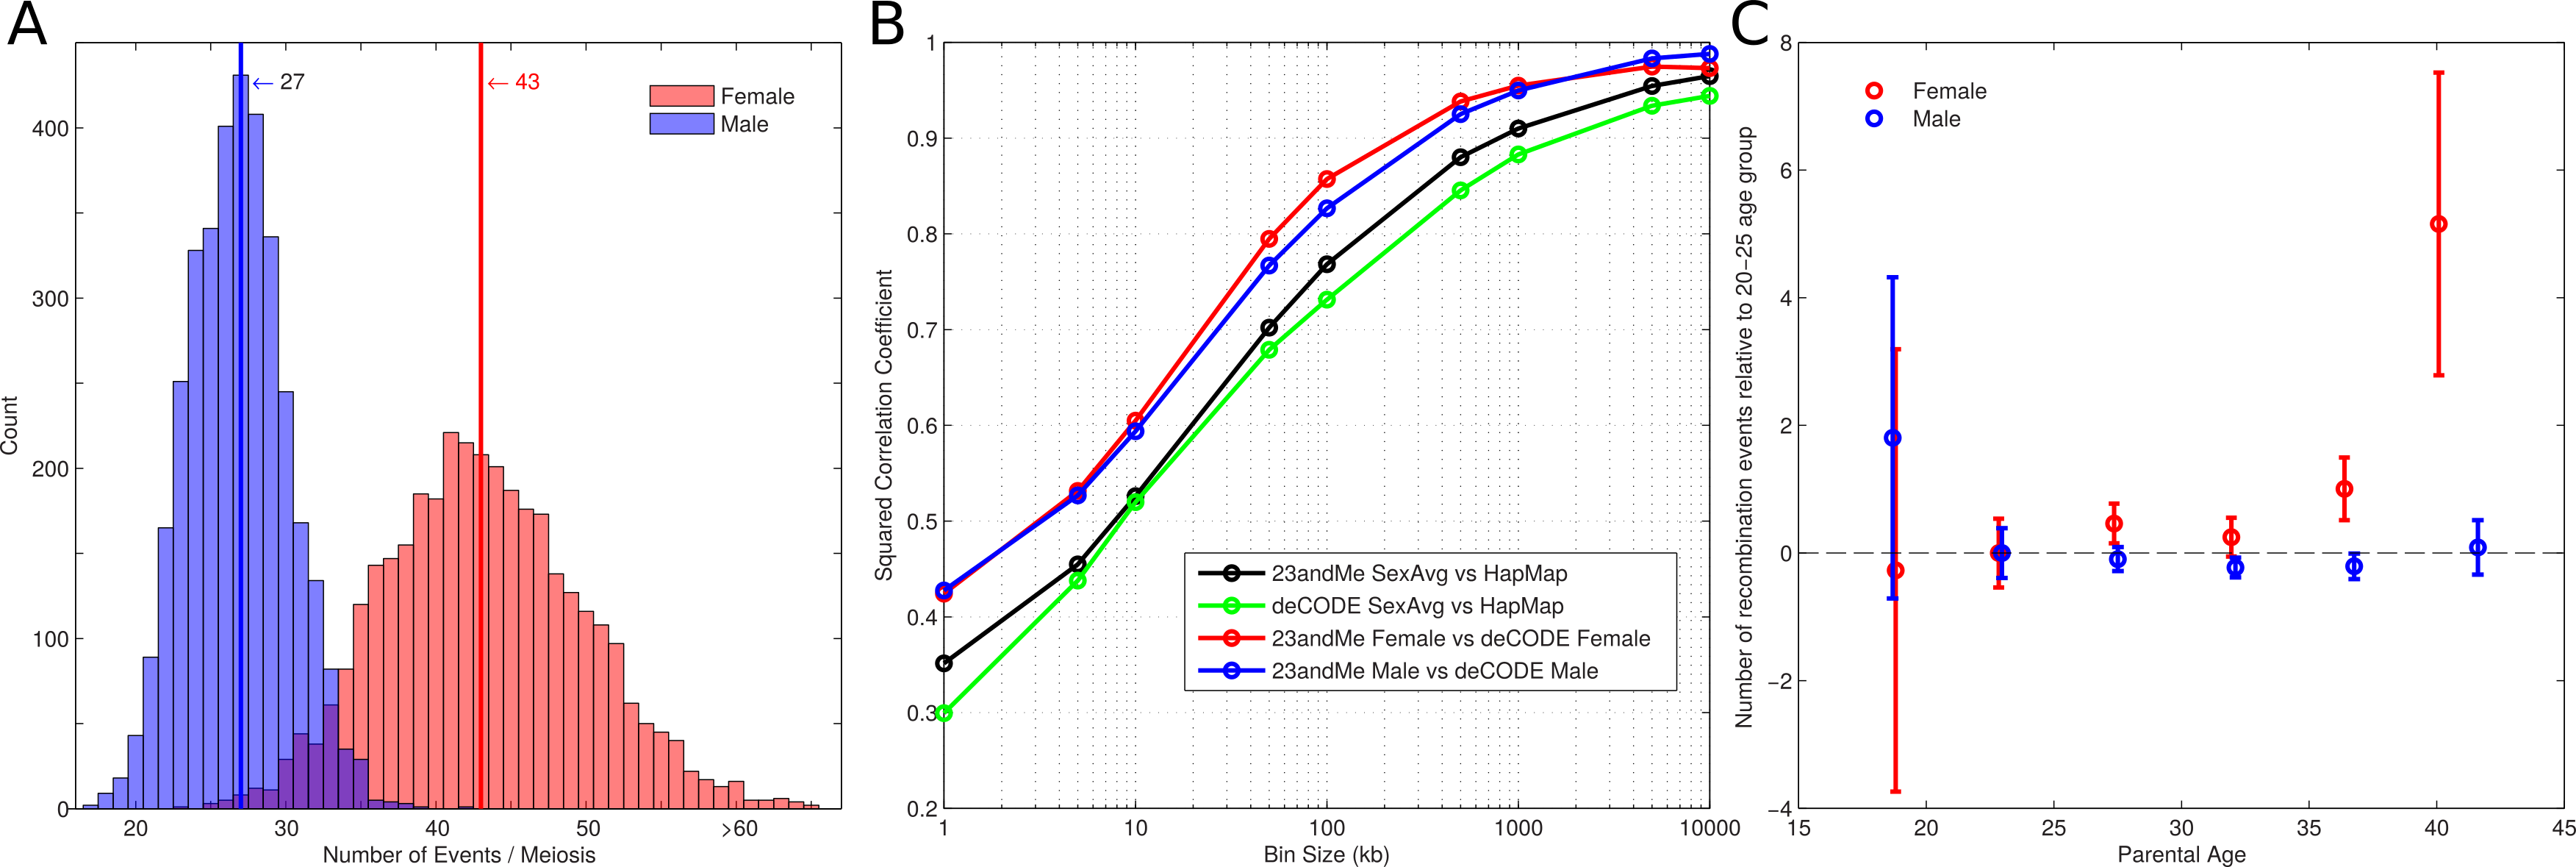
\includegraphics[width=\textwidth]{cointEscape/figs/Figure1.png}
    \vspace{-20pt}
    \captionTitle{\textbf{Properties of recombination partitioned by sex and age.}}{ 
        (a) The number of events per meiosis for females (red, n $=$ 9152) and males (blue, n $=$ 9150), with median values indicated by a vertical line. For phase-unknown individuals, the average number of events per meiosis was used. 
        (b) Squared Pearson correlation between the 23andMe map, the deCODE map and the HapMap map, as a function of scale. 
        (c) The number of recombination events as a function of parental age for females (red, n $=$ 9152) and males (blue, n $=$ 9150), relative to parents of between 20 and 25 years of age. Parents were grouped into 5-year age bins, and the mean number of events estimated. Error bars show a 95\% confidence interval for each group.
    \label{fig:cointF1}}
\end{figure}

Treating the overall recombination rate as a phenotype, we
replicate genetic associations at genome-wide significance for
RNF212, which is known to be essential for crossover-specific
complexes\cite{Reynolds2013}, and within the vicinity of TTC5, which appears
to replicate an association with CCNB1IP1 (\citet{Kong2014}). Another
association near SMEK1 also replicates discoveries elsewhere\cite{Kong2014},
but not at genome-wide significance (Supplementary Table 4).

Previous reports have suggested increased recombination rates
in older females\cite{Kong2004,Coop2008}. Using linear regression (Supplementary
Fig. \ref{fig:cointFS6}), we obtain a similar result with an additional 0.067
events per year being observed in females ($P=$ 0.002, F-test), and
no such effect being observed in males ($P=$ 0.30, F-test). The
female effect appears to be driven by sharp increase in the
number of recombination events for older mothers (Fig. \ref{fig:cointF1}c).
Fitting the piecewise-linear model with a single change point
infers a rapid increase in the female recombination rate after 38.8
years, increasing from 0.047 events per year to 2.990 events per
year. On average, mothers of 39 years and over have an additional
2.51 events compared with younger mothers ($P=$ 0.0005,
Mann-Whitney U).

One possible interpretation of the increasing number of
recombination events with maternal age is that mothers with
higher recombination rates can maintain fertility until a later
age\cite{Kong2004} . To investigate this possibility, we focused on 776 mothers
(providing 2,184 meioses) that were part of larger families and
could have recombination events assigned to specific children.
After subtracting off the average age and average number of
recombination events for each mother, the resulting regression
does not find a significant association with age ($P=$ 0.11, F-test),
although we estimate our power to detect an effect size of an
additional 0.067 events per year in this subsample to be no more
than 30\%.

Both pedigree and LD studies have suggested that $\sim$60-70\% of
crossover events occur within recombination hotspots\cite{Coop2008,Myers2005}. Our
data confirm this result with 62.7\% of events occurring within
LD-defined hotspots in females, and 67.3\% occurring within
hotspots in males (Fig. \ref{fig:cointF2}a; Supplementary Fig. \ref{fig:cointFS7}A). The 4.6\%
difference between the two sexes is highly significant
($P=$ \num{1.1e-69}, Mann-Whitney U), suggesting differences in
the regulation of crossover placement between the sexes. The
result remains significant after thinning the female data to match
the crossover density of the male data ($P<$ \num{2.2e-16},
Mann-Whitney U), and does not appear to be driven by
increased male recombination rates near the telomeres (see
Supplementary Methods).

Hotspot localization is believed to be under the control of the
zinc-finger protein PRDM9, which recognizes and binds specific
DNA motifs\cite{Berg2010,Berg2011,Hinch2011,Parvanov2010}. We find single-nucleotide polymorphisms
(SNPs) in the vicinity of PRDM9 to be strongly associated with
the degree of hotspot usage, as has previously been reported\cite{Kong2014,Hinch2011}.
The most strongly associated SNP is rs73742307 achieving a
P value of \num{7.9e-184} (\citet{Reynolds2013}), with no other region achieving a
genome-wide significant association with this phenotype
(Supplementary Table 5).

Variation within the PRDM9 DNA-binding domain can result
in changes to the recognized motif and hence lead to differences
in hotspot localization between individuals. While the major allele
of PRDM9 (allele A) is present at high frequency in most human
populations, a large number of low-frequency alleles have been
observed, particularly within African populations\cite{Berg2011,Parvanov2010}. Consistent
with this, we find hotspot usage to be significantly lower within
individuals of African ancestry (Fig. \ref{fig:cointF2}b; Supplementary Table \ref{tab:cointTS6}),
which reflects the fact that the LD-defined hotspots are expected
to mostly represent the common PRDM9 allele. Notably, while
over 75\% of our data are derived from individuals of European
ancestry, hotspot usage is higher for males than females across all
ancestries.

\begin{figure}[h]
    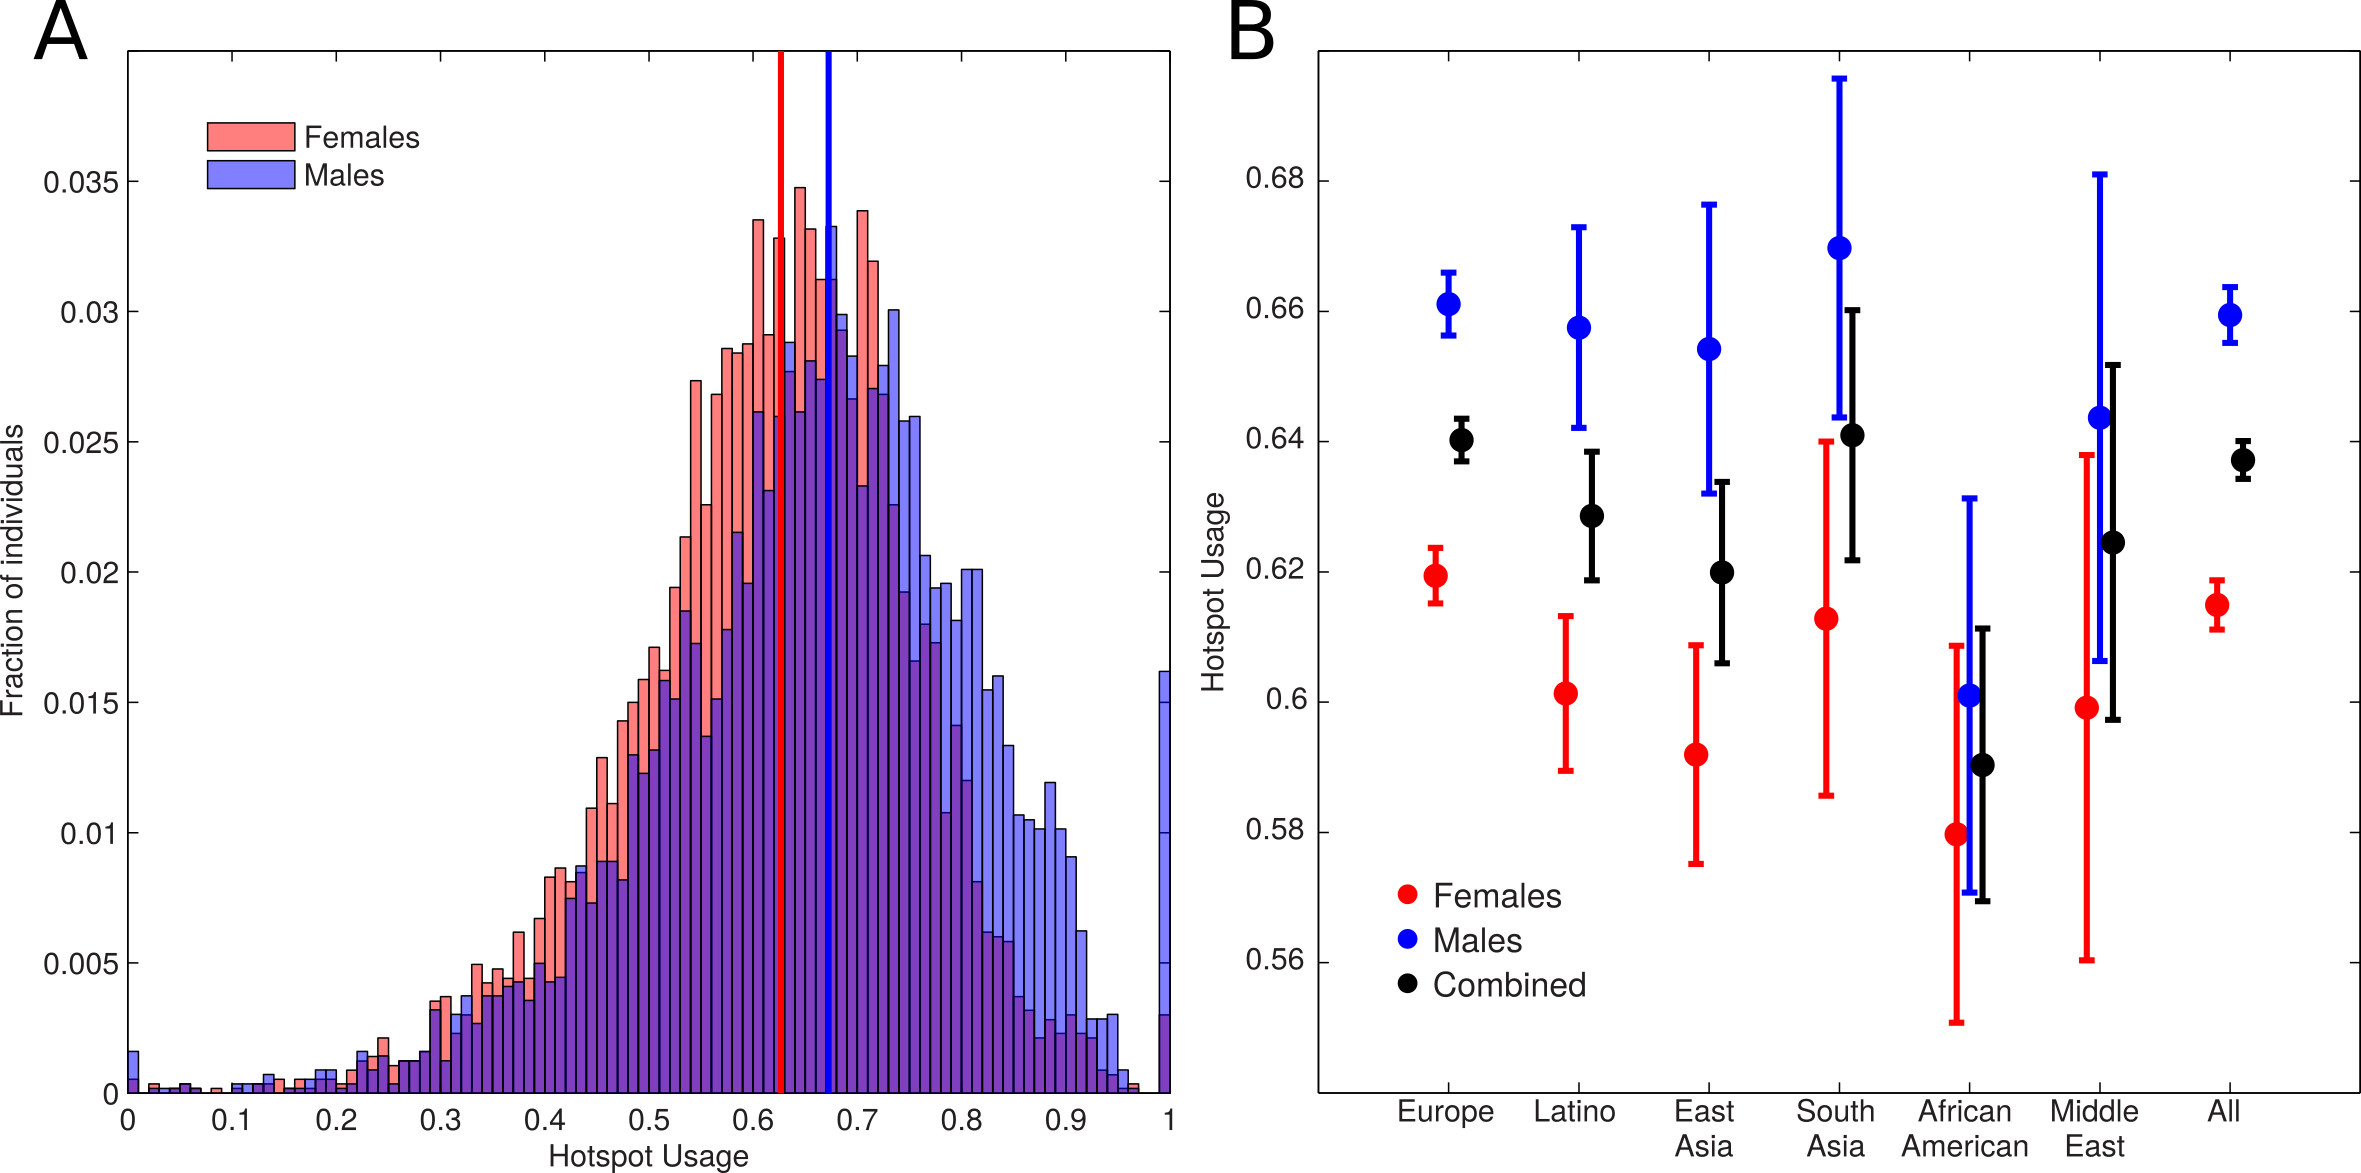
\includegraphics[width=\textwidth]{cointEscape/figs/Figure2.png}
    \vspace{-20pt}
    \captionTitle{\textbf{Sex differences in recombination hotspot usage.}}{
        (a) Hotspot usage for female (red, n $=$ 9152) and male (blue, n $=$ 9150) meioses. Median values for each sex are shown by vertical lines. 
        (b) Mean hotspot usage, subdivided by parental population. Females are shown in red, males in blue and a combined estimate in black. Error bars indicate a 95\% confidence interval.
       \label{fig:cointF2}}
\end{figure}

We find a weak association between hotspot usage and
maternal age (Supplementary Fig. \ref{fig:cointFS7}B). Using logistic regression,
we estimate a decrease in hotspot usage corresponding to
$\sim$1\% over a 10-year period ($\beta_1=$ \num{-0.0042}, $\text{s.e.}=$ \num{9.6e-4}, 
$P=$ \num{1.2e-5}, F-test). To ensure this effect is not driven by
differences in parental ancestry within the sample, we repeated
the analysis only using individuals of European ancestry. In this
case, the effect size remains similar ($\beta_1=$ \num{-0.0033}, $\text{s.e.}=$ 0.0013),
but is only marginally significant ($P=$ 0.0101, F-test). Including
the number of events as an additional predictor variable within
the regression leaves age as a weakly significant predictor
($P=$ 0.0106, F-test), but not the number of events ($P=$ 0.74,
F-test). Despite the small size of the estimated effect, we note that
no such age-related effects were observed in males.

To learn more about interactions between recombination
events, we used the high number of crossover locations in our
data to better characterize the phenomenon of crossover
interference. By considering the distribution inter-crossover
distances, we fit three models to describe the distribution of
inter-crossover distances: a model without interference between
crossovers (also known as the gamma model of crossover
interference\cite{Broman2000}), and a mixture model in which a subset of
events come from a process that exhibits no interference (also
known as the Housworth-Stahl model\cite{Housworth2003}). To fit these models, we
used existing methods for families in which recombination events
could be assigned to specific individuals, and extended these
methods for smaller families where recombination events cannot
be simply assigned to a specific individual (see Supplementary
Methods).

In agreement with previous reports\cite{Housworth2003,Fledel-Alon2009}, the Housworth-Stahl
interference escape model provides a much better fit to our
data than either the gamma simple interference model or the
interference-free model (Fig. \ref{fig:cointF3}a). Under this model, the estimates
of the strength of crossover interference are similar to previous
reported using smaller data sets\cite{Fledel-Alon2009}. The degree of interference is
inferred to be lower in females than in males ($\nu_{female}=$ 7.19 vs
$\nu{male}=$ 8.93). In addition, 7.8\%/6.7\% of female/male events are
inferred to escape interference. We therefore conclude that a
non-negligible fraction of crossovers occur in the absence of
crossover interference.

We find evidence that both the degree of interference and
interference escape varies across chromosomes (Fig. \ref{fig:cointF3}b,c;
Supplementary Table \ref{tab:cointTS7}). The strength of interference is reasonably 
well predicted by the chromosome map length ($r^2=$ 0.565,
$P=$ \num{6.4e-9}), although the relationship is only significant in
females when considering the sexes separately ($r^2_{female}=$ 0.69,
$P=$ \num{1.7e-6} and $r^2_{male}=$ 0.172, $P=$ 0.06; Supplementary Fig. \ref{fig:cointFS8}).
In contrast, the fraction of events escaping interference shows no
relationship with chromosome map length ($r^2=$ 0.001, $P=$ 0.84).
Certain chromosomes appear to have high degrees of escape, with
chromosomes 8, 9 and 16 (in females) being notable outliers.

\begin{figure}[h]
    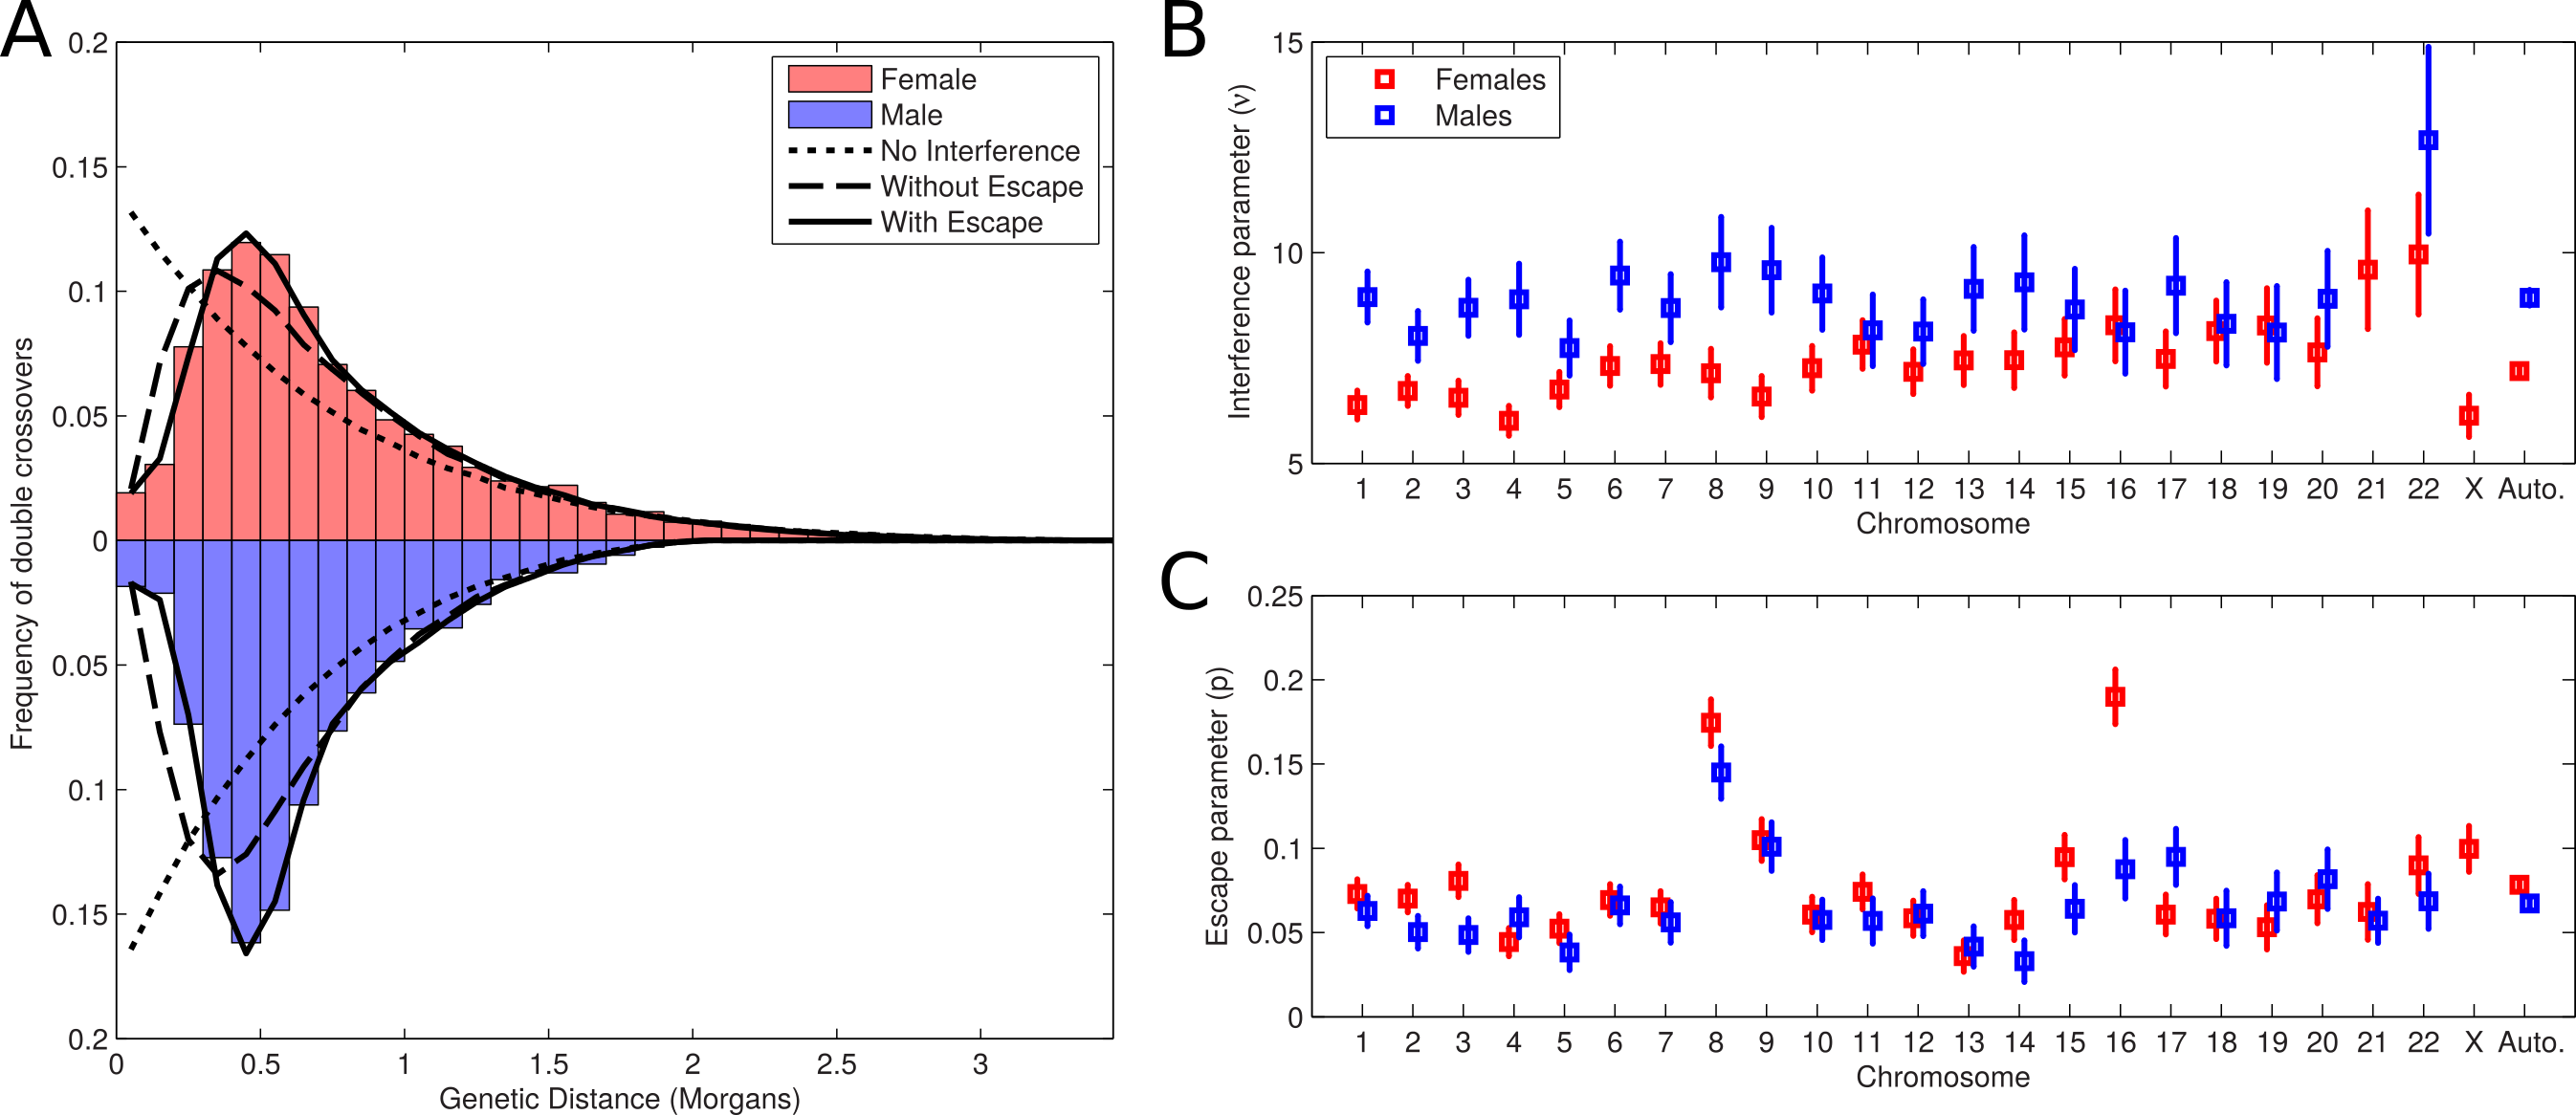
\includegraphics[width=\textwidth]{cointEscape/figs/Figure3.png}
    \vspace{-20pt}
    \captionTitle{\textbf{Estimation of crossover interference parameters.}}{
        (a) Fit of three models of interference to the inter-crossover distances observed on chromosome 1, derived from phase-known mothers (red, n $=$ 2184) and fathers (blue, n $=$ 2092).
        The interference-free model is shown as a dotted line, the gamma simple interference model is shown as a dashed line and the Housworth-Stahl interference escape model is shown as a solid line. 
        (b) Per-chromosome estimates of the interference parameter as estimated from the Housworth-Stahl interference escape model.
        Error bars indicate a 95\% confidence interval.
        Note that chr21 in males is excluded due to an extremely high estimate.
        (c) Per-chromosome estimates of the proportion of events escaping interference. Error bars indicate a 95\% confidence interval.
       \label{fig:cointF3}}
\end{figure}

To investigate whether crossover interference changes with
parental age, we subdivided our data into 10 quantiles on the
basis of age, and fit the Housworth-Stahl interference escape
model to each group independently. We observe a striking
increase in the proportion of events that escape interference with
maternal age (Fig. \ref{fig:cointF4}a), rising from 6.7\% for mothers under 25
years to 9.5\% for mothers over 35 years. No such correlation is
observed for the interference parameter in females, and no
correlation is observed for either parameter in males
(Supplementary Fig. \ref{fig:cointFS9}). The effect is robust to different subdivisions % edited typo
of the data (Supplementary Figs \ref{fig:cointFS10} and \ref{fig:cointFS11}).

A potential concern is that the detected increase in interference
escape could be driven by the observed increased number of
crossovers in older mothers. If the number of crossovers is 
increased, then the distances between them are necessarily
shorter, which may in turn influence the interference parameter
estimates. To account for this possibility, we performed stratified
sampling of individuals to control for the number of events
within each quantile. The observed increase in the escape
parameter with maternal age is still observed (Supplementary
Fig. \ref{fig:cointFS12}), indicating that it is not driven by changes in the overall
recombination rate.

To further investigate the differences between old and young
parents, we plotted the distribution of inter-crossover distances
for young and old parents (Fig. \ref{fig:cointF4}b,c). The interference escape
effect in females appears to be predominately driven by an
increase in the number of very tightly clustered events, generally
separated by less than $\sim$5 cM. These tightly clustered events are
not well captured by the Housworth-Stahl interference escape
model (Supplementary Fig. \ref{fig:cointFS13}), and a major concern therefore is
that these tightly clustered events represent false-positive calls
arising from genotyping error. However, the effect remains even
if we apply much stricter filtering of the crossover events
(Supplementary Fig. \ref{fig:cointFS14}), and in addition we believe genotyping
error is unlikely to explain the association between the escape
parameter and maternal age because (a) the effect is not seen in
males, and (b) it would imply increased genotyping error for
older mothers (but not fathers).

\begin{figure}[h]
    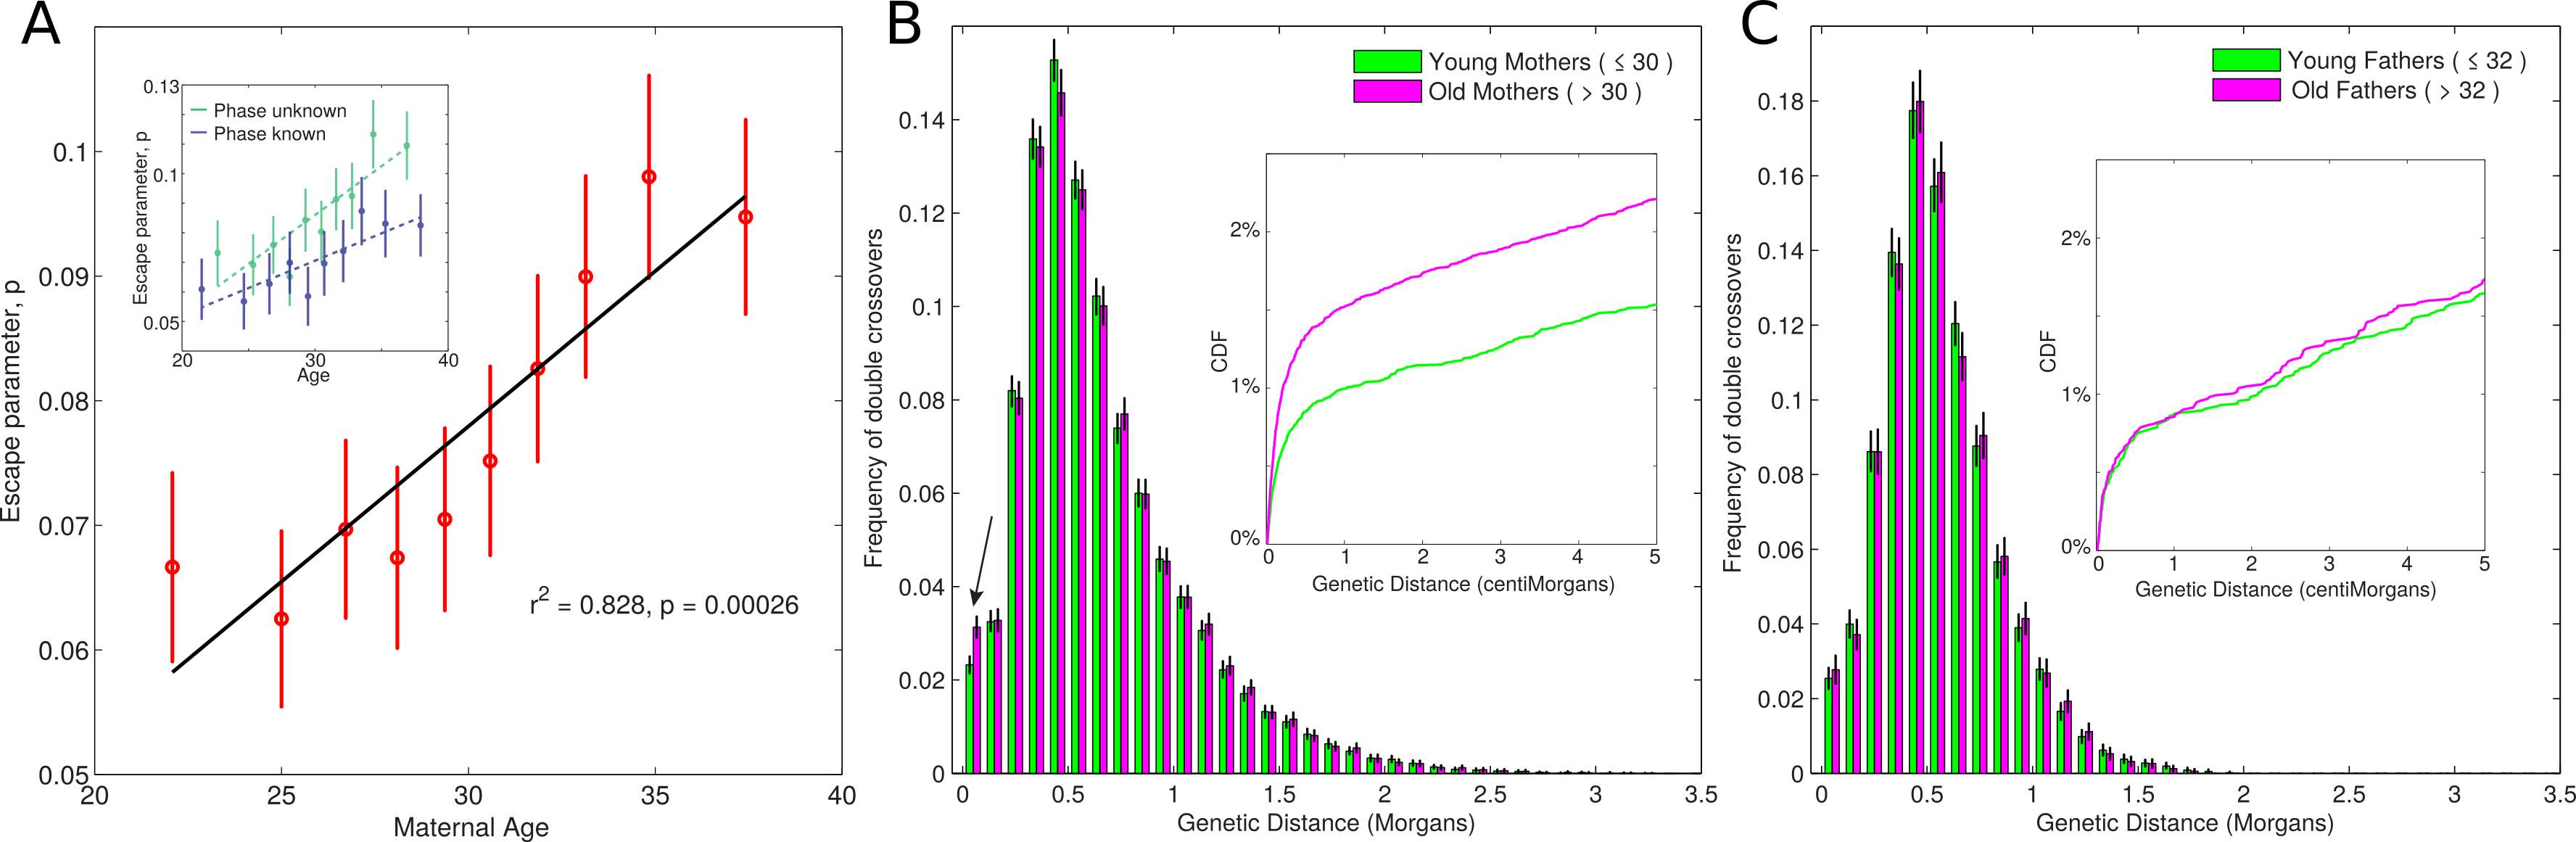
\includegraphics[width=\textwidth]{cointEscape/figs/Figure4.png}
    \vspace{-20pt}
    \captionTitle{\textbf{Departures from simple crossover interference.}}{
        (a) Inferred escape parameter as a function of maternal age.
        Mothers were divided into 10 approximately equal-sized deciles on the basis of age, and the Housworth-Stahl interference escape model was fitted for each group separately.
        The inset shows the estimates of the escape parameter when considering phase-known (blue, n $=$ 2184) and phase-unknown (green, n $=$ 6968) individuals separately. 
        Estimates for $\nu$ show no correlation with age (Supplementary Fig. \ref{fig:cointFS9}). Error bars indicate 95\% confidence intervals. 
        (b) Distribution of inter-crossover distances for young and old mothers, where the boundary between young and old is taken as median maternal age (30 years). 
        Error bars represent a 95\% confidence interval assessed via 1000 bootstrap samples, and the arrow highlights a significant difference between the young and old groups for tightly clustered events. 
        The inset shows the cumulative distribution function (CDF) up to 5 cM. 
        (c) Distribution of inter-crossover distances for young and old fathers, where the boundary between young and old is taken as median paternal age (32 years).
       \label{fig:cointF4}}
\end{figure}

In terms of meiosis, a major difference between the sexes is that
female meiosis starts during fetal development, but does not
complete until adulthood. As such, while male gametes are
produced throughout adulthood and promptly proceed through
meiosis, oocytes remain arrested in a late stage of prophase
(dictyotene) for many years, if not decades. Presuming our
observation of increasing crossover interference escape with
maternal age is not due to some obscure form of genotyping
error, our observations add to similar evidence of increasing rates
of recombination\cite{Kong2004} and aneuploidy\cite{Hassold2001} in aging females. Although
these phenomena are presumably related, the biological
mechanisms by which they occur are unclear, and we can think
of at least three possibilities. First, given chromatids remain
physically proximal during the extended period of female meiotic
arrest, one possible explanation is that additional recombinations
are initiated during this time, perhaps in response to
DNA damage. However, as recombination is believed to have
completed by the time of dictyotene, such an explanation appears
unlikely. A second possibility, previously invoked to explain the
increasing recombination rate with maternal age\cite{Kong2004}, suggests
oocytes with additional recombination events could be at
reduced risk of nondisjunction, and hence would be more likely
to lead to viable embryos in older mothers. However, it is not
clear that this mechanism would explain the increased clustering
of events observed in our data. Finally, a third possibility is 
related to the so-called ``production line'' hypothesis, in which
oocytes are selected for maturation sequentially in the same order
as their generation, and later oocytes have therefore potentially
undergone additional mitotic divisions prior to entering
meiosis\cite{Reizel2012}. However, the existence of a production line has been
debated for many years\cite{Reizel2012,Polani1991,Rowsey2014}, and so the likelihood of this
explanation is unclear.

%%%%%%%%%%%%%%%%%%%%%%%%%%%%%%%%%%%%%%%%
%%%%%%%%%%%%%%%%%%%%%%%%%%%%%%%%%%%%%%%%
\section{Methods}
%%%%%%%%%%%%%%%%%%%%%%%%%%%%%%%%%%%%%%%%
%%%%%%%%%%%%%%%%%%%%%%%%%%%%%%%%%%%%%%%%

\paragraph{Sample genotyping.} Samples were collected and genotyped at the consumer
genetics company 23andMe Inc., as described previously\cite{Eriksson2010}. Briefly, genotyping was
performed on genomic DNA extracted from saliva samples. DNA was genotyped
on one of two microarray platforms: the Illumina HumanHap550+ BeadChip
platform, which includes more than 550,000 SNPs, or the Illumina
HumanOmniExpress+ BeadChip, which has a base set of 730,000 SNPs
augmented with $\sim$250,000 SNPs to obtain a superset of the HumanHap550+,
as well as a custom set of about 30,000 SNPs.

\paragraph{Pedigree construction.} Pedigrees were constructed first by identifying trios using
estimated identity-by-decent relationships. Trios were then combined to form
nuclear families, and nuclear families were joined based on the assumed
relationships to form larger pedigrees. We identified trios by finding triplets of
individuals in the 23andMe customer cohort that had estimated identity-by-decent
relationships matching those expected in a true trio. Trios were accepted if both
parents were at least 18 years old upon the birth of the child and one parent was
male and the other female. We created nuclear families by identifying all trios with
the same two parents and then by combining the children of these trios. Finally,
larger pedigrees were created by simply joining the nuclear families based on the
assumed relationships and by accounting for directionality given by the age of
individuals. Any two individuals with more than one potential relationship were
excluded along with the pedigrees they belonged to.

\paragraph{Calling of recombination events and data filtering.} Prior to data filtering,
the data set consisted of 4,270 pedigree families, with data pertaining to 18,647
informative meioses. This raw data set consisted of 692,876 recombination events,
with a median of 45 and 28 events per meiosis in females and males, respectively.

The Merlin algorithm (version 1.1.2) used to detect recombination events does
not account for genotyping error, and genotyping errors are therefore likely to
result in spurious recombination event calls. To account for this issue, our first step
was to only use high-confidence sites. First, we required the sites to have a call rate
greater than 90\% and Hardy-Weinberg $P$ value $\le$ \num{1e-20} (as calculated in the
23andMe cohort). Second, we excluded sites with minor allele frequencies differing
from those of the 1000 Genomes Phase 1 reference panel\cite{1000G2012}. This was achieved by
constructing a 2 $\times$ 2 contingency table and comparing the 1000 Genomes
European allele counts with those from 2,000 randomly selection 23andMe
customers, and using a $\chi^2$-test to identify significant deviations. Sites with $P$ values
less than \num{1e-15} were removed.

Having applied these basic site filters, we next aimed to remove any weakly
supported recombination events. This was achieved by first using the Merlin ``error''
feature to remove potential genotyping errors not consistent with gene flow within
each pedigree. In addition, we excluded all recombination events supported by less
than three recombination-informative sites on either side, where we define an
informative site as a site that is called as heterozygotic in exactly two individuals
out of each mother-father-child trio. Finally, we removed all pairs of events within
each single family that occurred within the same SNP interval. Together, these
filters removed 31,742 weakly supported events, which corresponded to 4.6\% of the
total number.

Preliminary inspection of the genetic maps identified a region on chromosome
10 where the 23andMe genetic map diverged substantially from that generated by
deCODE\cite{Kong2010}. This can be seen in a plot of the chromosome 10 genetic map at
$\sim$50 Mb (Supplementary Fig. \ref{fig:cointFS2}A).

Further investigation of this region revealed a large number of ``double''
crossovers in close proximity to each other (that is, pairs of recombination events
occurring in close proximity within the same individual). While some such
observations are expected through the action of gene conversion, such strong
clustering of these events is not expected biologically. Instead, we believe the result
is suggestive of misplacement of polymorphisms, mis-assembly of one or more
reference contigs in the hg19 reference genome or of more complex types of
error related to copy number polymorphism or array design. In any case, these
double-recombination events represent a form of error that needed to be
eliminated.

To better quantify this issue, we identified all pairs of recombination events
occurring within a single individual that were within 1 Mb of each other. For each
SNP in the genome, we estimated the number of these event pairs that span the
SNP (Supplementary Fig. \ref{fig:cointFS2}B).

For the vast majority of the genome, there were very few such event pairs, and
hence localized peaks likely represent data quality issues. We therefore identified all
SNPs spanned by at least 14 event pairs (with this threshold being equivalent 
to the 99.9th percentile of the distribution). In this way, we identified 50 regions
with strong enrichment of nearby event pairs (Supplementary Table 8). Note that
for this analysis we ignored the pseudoautosome, as a large number of events
occurring in close proximity might be expected due to the extreme male
recombination rate within this region.

The regions with high numbers of clustered events were themselves clustered
into 13 regions across 8 chromosomes, and are often in the vicinity of chromosome
centromeres, telomeres or reference assembly gaps. We removed all event pairs
within 500 kb of the region boundaries described in Supplementary Table 8, which
resulted in the removal of 2,916 events (0.42\% of the total). The removal of these
events improved the concordance between the 23andMe and deCODE maps
(Supplementary Fig. \ref{fig:cointFS2}C).

Previous research using well-curated data in 728 meioses reported an average of
39.6 autosomal events per gamete in females (95\% CI 38.5-40.6), and 26.2
autosomal events per gamete in males (95\% CI 25.6-26.7)7. The minimum/
maximum number of observed autosomal events in any given meiosis in this
data was 19/71 for females, and 16/43 for males (Graham Coop, personal
communication).

Preliminary analysis of our data revealed a small subset of individuals had
biologically unrealistic numbers of recombination events. Our first filtering step
was to remove the pedigrees containing these individuals. Specifically, we removed
individuals (and their containing pedigrees) that were more than 5 s.d. from the
(sex specific) median number of recombination events. To guard against outliers,
we used a robust estimate of the s.d. taken as $\sigma=$ 1.4826 MAD, where MAD
represents the median absolute deviation.

Before filtering, the median number of recombination events was 43 and 27 for
females and males, respectively (including chrX and the pseudoautosome). Using
the $\pm$5$\sigma$ thresholds, we removed pedigrees containing any female with fewer than
10 or more than 76 events per meiosis, or any male with fewer than 9 or more than
45 events. These filters removed a total of 52 pedigrees.

\paragraph{Summary of the filtered data set.} After applying the filtering steps described
above, the filtered data set consists of 4,209 pedigrees containing 18,302
informative meioses, of which 9,152 are from females and 9,150 are from males.
Of the families included in the study, 78.6\% are family quartets, 14.3\% are larger
one-generation families, and 7.1\% are two-generation families (Supplementary
Table 1).

Due to the structure of the pedigrees included in the study, certain
recombination events can be identified as having occurred within a specific child,
whereas others cannot. For example, in family quartets, it is generally unclear
which child has the recombinant haplotype, and we therefore refer to these events
as ``phase unknown''. Conversely, the child containing the recombinant haplotype
can generally be identified in larger pedigree families in which the parental
haplotype can be confidently phased, and we therefore refer to these events as
``phase known''.

In total, 4,276 meioses are derived from phase-known individuals, whereas
14,026 are derived from phase-unknown individuals. Of the female meioses, 2,184
are derived from phase-known mothers and 6,968 are from phase-unknown
mothers. Of the male meioses, 2,092 are derived from phase-known fathers, and
7,058 are derived from phase-unknown fathers.

Individuals were assigned to high-level population groups via comparison with
a set of reference populations (see Supplementary Methods). The majority of
individuals in the data set are of European descent, with $\sim$78\% of the meioses in
the sample occurring within a European individual (Supplementary Table 2).

The parental age distribution for the filtered data set is shown in Supplementary
Fig. \ref{fig:cointFS1}. The mean age was 30 years for females, and 32 for males.

The final filtered data set consists of 645,853 recombination events. Including
the sex chromosomes, the mean number of recombination events was 43.47 for
females ($\sigma=$ 6.64, 95\% CI 43.25-43.69), and 27.04 for males ($\sigma=$ 3.28, 95\% CI
26.94-27.16). For the autosomes alone, the mean number of recombination events
was 41.64 for females ($\sigma=$ 6.34, 95\% CI 41.43-41.85) and 26.61 for males
($\sigma=$ 3.26, 95\% CI 26.51-26.73).

The distribution of interval sizes to which crossovers could be resolved (that is,
the distance between informative markers on either side of the recombination
event) is given in Supplementary Fig. \ref{fig:cointFS3}. Crossovers could be resolved within a
median distance of 28.2 kb.

%%%%%%%%%%%%%%%%%%%%%%%%%%%%%%%%%%%%%%%%
\section{Acknowledgements}
%%%%%%%%%%%%%%%%%%%%%%%%%%%%%%%%%%%%%%%%
We would like to thank Hilary Martin and Julie Hussin for their constructive comments
regarding earlier versions of this manuscript. C.L.C. was supported by the Training
Program in Cellular and Molecular Biology and Genetics, T32 GM007491. Work by
N.A.F., N.E. and D.H. was supported by NIH award 2R44HG006981-02.

%%%%%%%%%%%%%%%%%%%%%%%%%%%%%%%%%%%%%%%%
\section{Author contributions}
%%%%%%%%%%%%%%%%%%%%%%%%%%%%%%%%%%%%%%%%
A.A., D.H. and N.E. designed the study. A.A., C.L.C. and N.A.F. conducted analysis.
A.A. and C.L.C. wrote the paper.

%%%%%%%%%%%%%%%%%%%%%%%%%%%%%%%%%%%%%%%%
\section{Additional information}
%%%%%%%%%%%%%%%%%%%%%%%%%%%%%%%%%%%%%%%%

\paragraph{Supplementary Information} accompanies this paper at \\ \url{http://www.nature.com/naturecommunications}

\paragraph{Competing Financial Interests:} N.A.F. and D.H. are current employees, and N.E. is a
former employee of 23andMe Inc., and have private equity interest. The remaining
authors declare no competing financial interests.

\paragraph{Reprints and permission} information is available online at \\
\url{http://npg.nature.com/reprintsandpermissions/}

\paragraph{How to cite this article:} Campbell, C. L. \textit{et al}. Escape from crossover interference
increases with maternal age. \textit{Nat. Commun.} 6:6260 doi: 10.1038/ncomms7260 (2015).

\bigskip \noindent
This work is licensed under a 
Creative Commons Attribution-NonCommercial-ShareAlike 4.0 International License. The images or
other third party material in this article are included in the article's Creative Commons
license, unless indicated otherwise in the credit line; if the material is not included under
the Creative Commons license, users will need to obtain permission from the license
holder to reproduce the material. To view a copy of this license, visit \\
\url{http://creativecommons.org/licenses/by-nc-sa/4.0/}

%%%%%%%%%%%%%%%%%%%%%%%%%%%%%%%%%%%%%%%%
%%%%%%%%%%%%%%%%%%%%%%%%%%%%%%%%%%%%%%%%
\bibliographystyle{ccampbell_thesis} %unsrtnat} %abbrvnat_noURL} %abbrvUnsrt_last-first} %plain,unsrt,alpha,abbrv,acm,apalike,unsrt
\bibliography{cointEscape/thesis-cointEscape}
%%%%%%%%%%%%%%%%%%%%%%%%%%%%%%%%%%%%%%%%
%%%%%%%%%%%%%%%%%%%%%%%%%%%%%%%%%%%%%%%%

%%%%%%%%%%%%%%%%%%%%%%%%%%%%%%%%%%%%%%%%
%%%%%%%%%%%%%%%%%%%%%%%%%%%%%%%%%%%%%%%%
\beginsupplement
\section{Supplementary Material}
%%%%%%%%%%%%%%%%%%%%%%%%%%%%%%%%%%%%%%%%
%%%%%%%%%%%%%%%%%%%%%%%%%%%%%%%%%%%%%%%%

\subsection{Supplementary Figures}

\begin{figure}[!h]
    %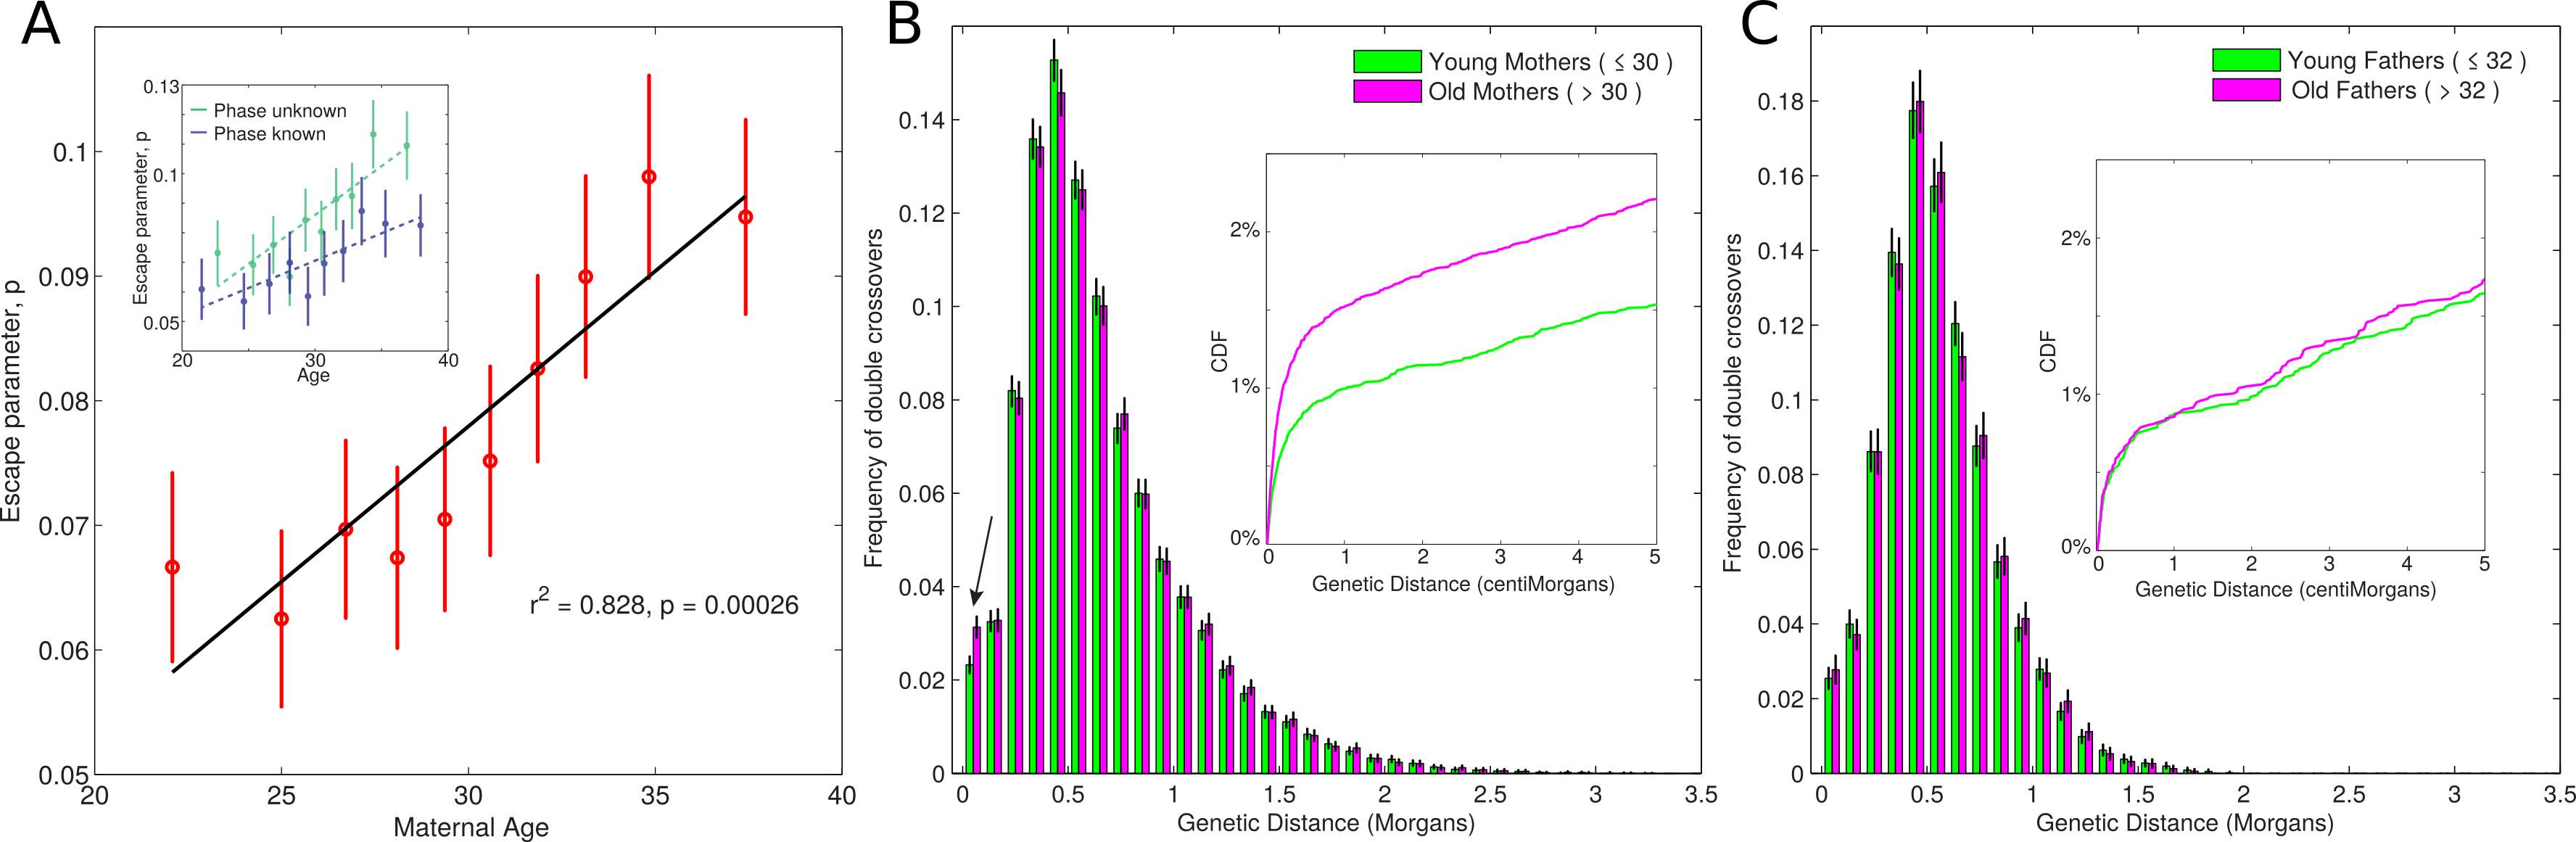
\includegraphics[width=\textwidth]{cointEscape/figs/Figure4.png}
    %\vspace{-20pt}
    \captionTitle{\textbf{Age distributions within the filtered dataset.}}{
        The left hand panel shows the distribution for phase-unknown individuals, where the parental ages were averaged across children. 
        The right hand panel shows data for the phase-known meioses where the parental age at the time of childbirth is known.
        Lines indicate the mean of each distribution. 
        Note that some families were excluded from analysis by 23andMe on the basis age to protect privacy, as seen from the truncated distribution of maternal ages in the right hand panel.  
       \label{fig:cointFS1}}
\end{figure}

\begin{figure}[!h]
    %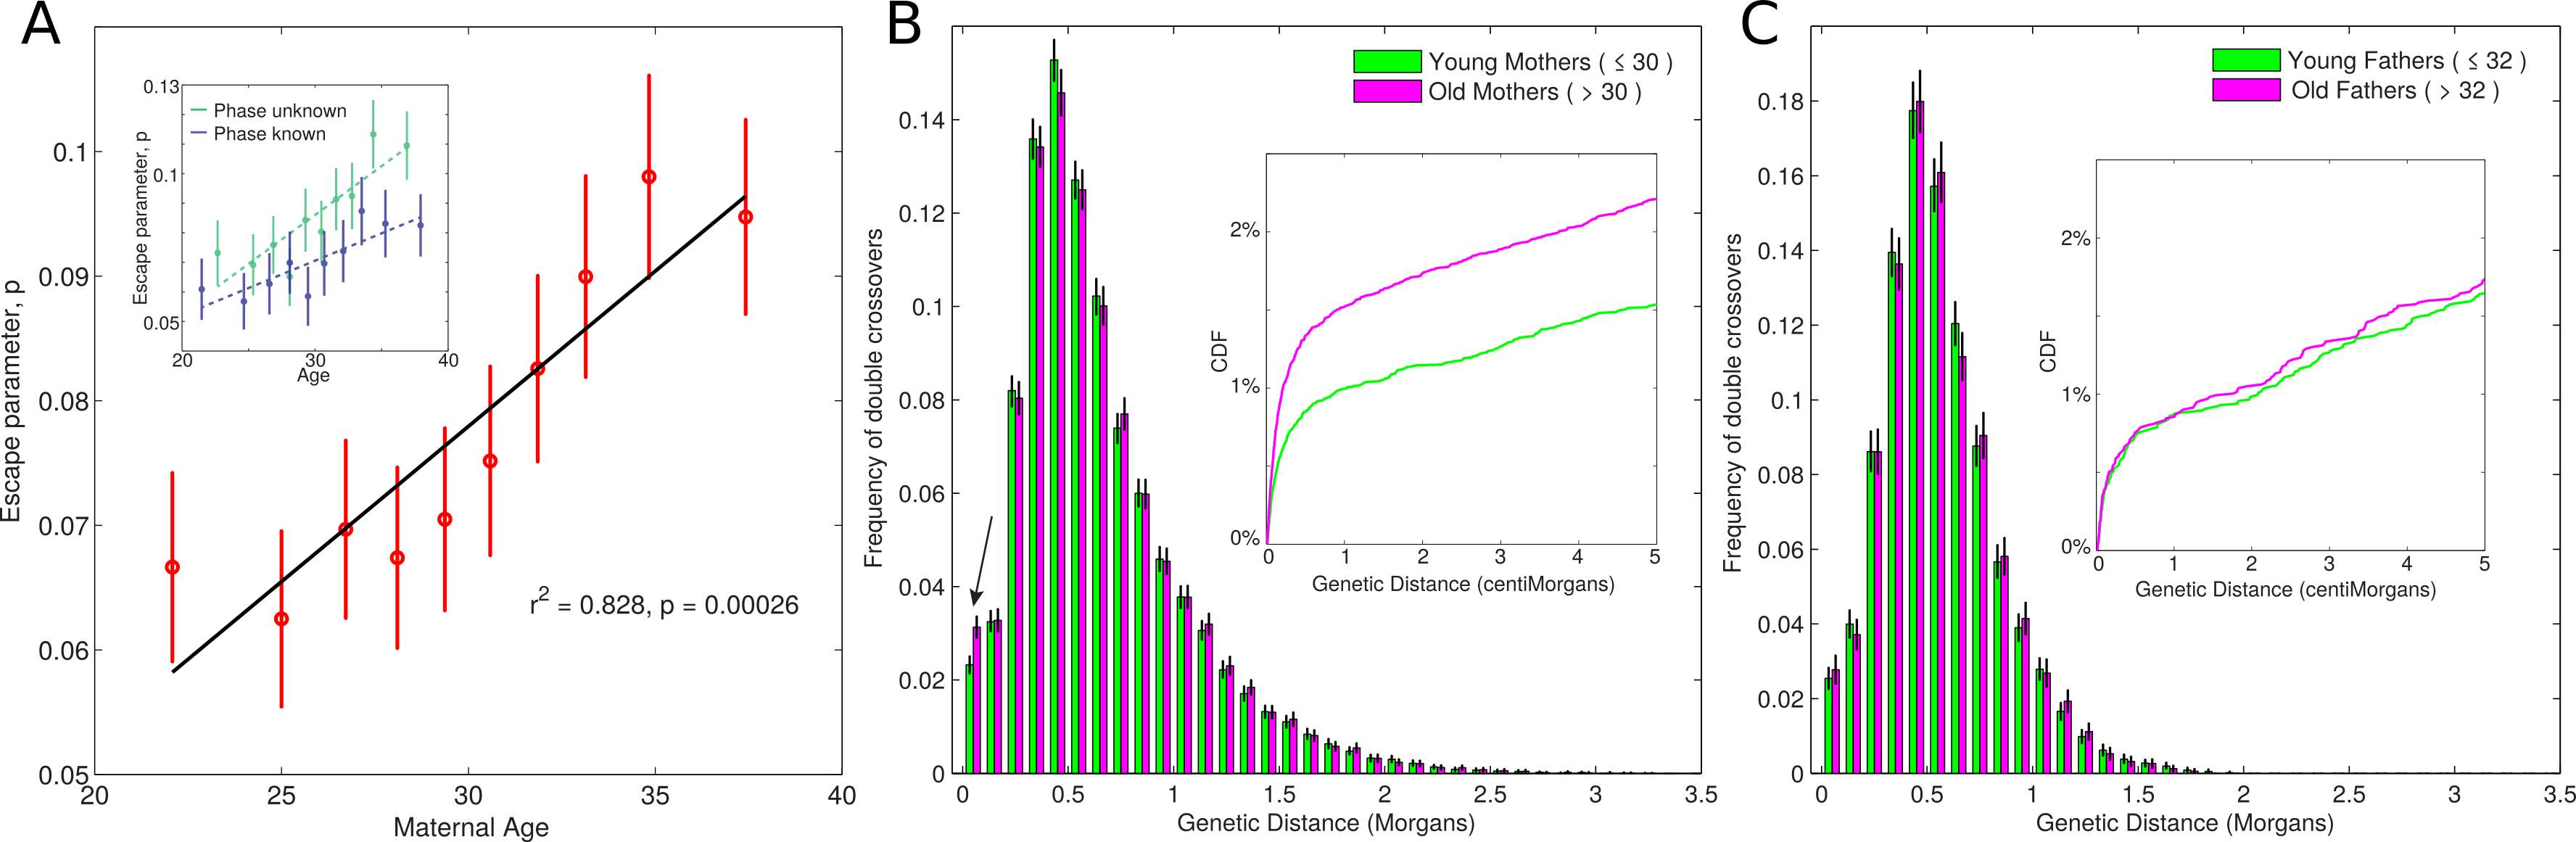
\includegraphics[width=\textwidth]{cointEscape/figs/Figure4.png}
    %\vspace{-20pt}
    \captionTitle{\textbf{Data grooming.}}{
        A) Chromosome 10 map before filtering.
        Genetic maps from the 23andMe data are shown in bold lines, whereas the genetic maps from deCODE are shown as thin lines.
        Separate maps are shown for females(red), males (blue), and sex-averaged (black). 
        Also shown are regions highlighted in grey that represent gaps in the reference assembly, the largest of which being the centromere at around 40Mb.
        B) Clustering of recombination events occurring within 1 Mb of each other within single individuals.
        Each plot shows the number of events within 1 Mb of each other on a log$_{10}$ scale as a function of physical position on each chromosome.
        A large number of these event pairs can be observed on chromosome 10, although other large peaks can also be observed on, for example, chromosomes 8 and 15.
        The dashed line represents the 99.9\% percentile of the distribution, and was used as a threshold for filtering.
        C) Chromosome 10 map after filtering.   
       \label{fig:cointFS2}}
\end{figure}

\begin{figure}[!h]
    %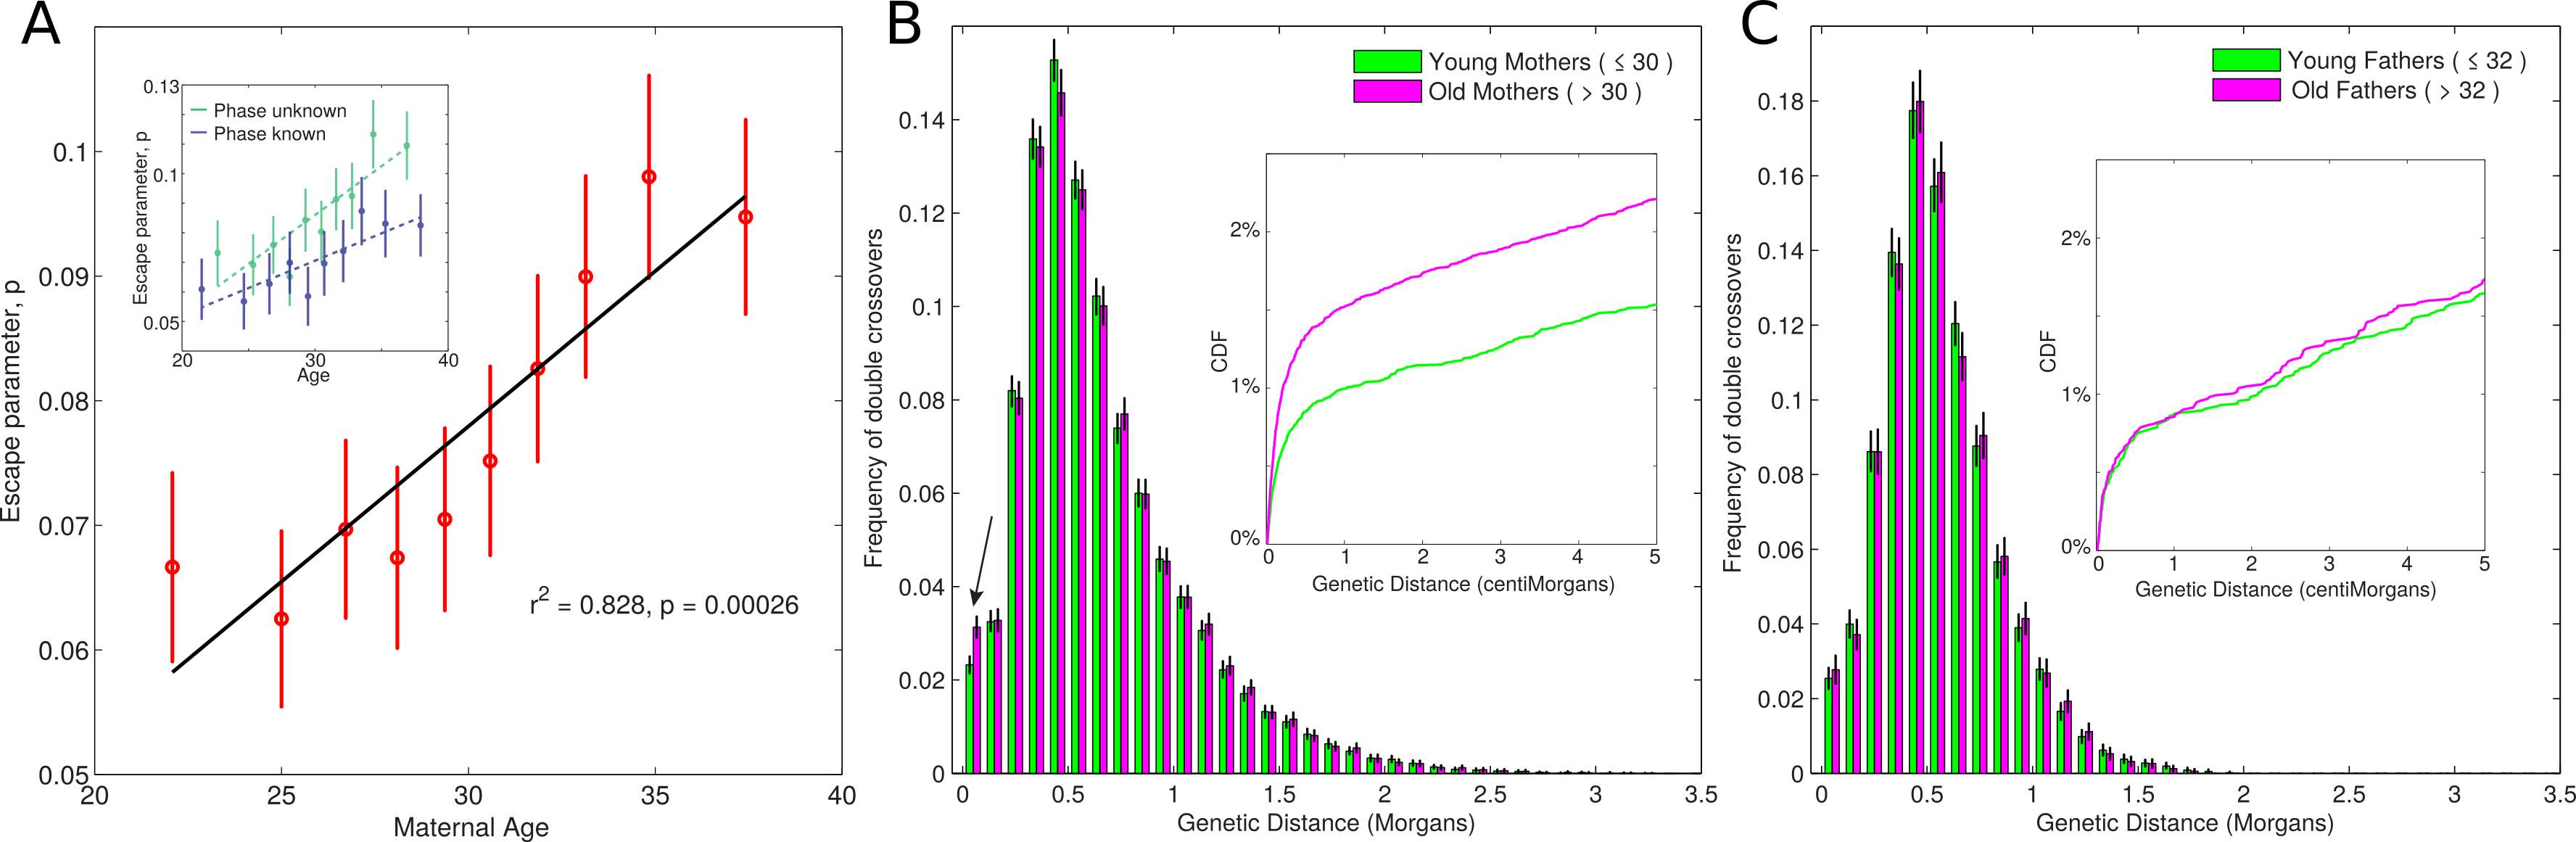
\includegraphics[width=\textwidth]{cointEscape/figs/Figure4.png}
    %\vspace{-20pt}
    \captionTitle{\textbf{Empirical cumulative distance function of crossover localization distances.}} { 
        Red labels indicate the interval distances at the distribution deciles.  
       \label{fig:cointFS3}}
\end{figure}

\begin{figure}[!h]
    %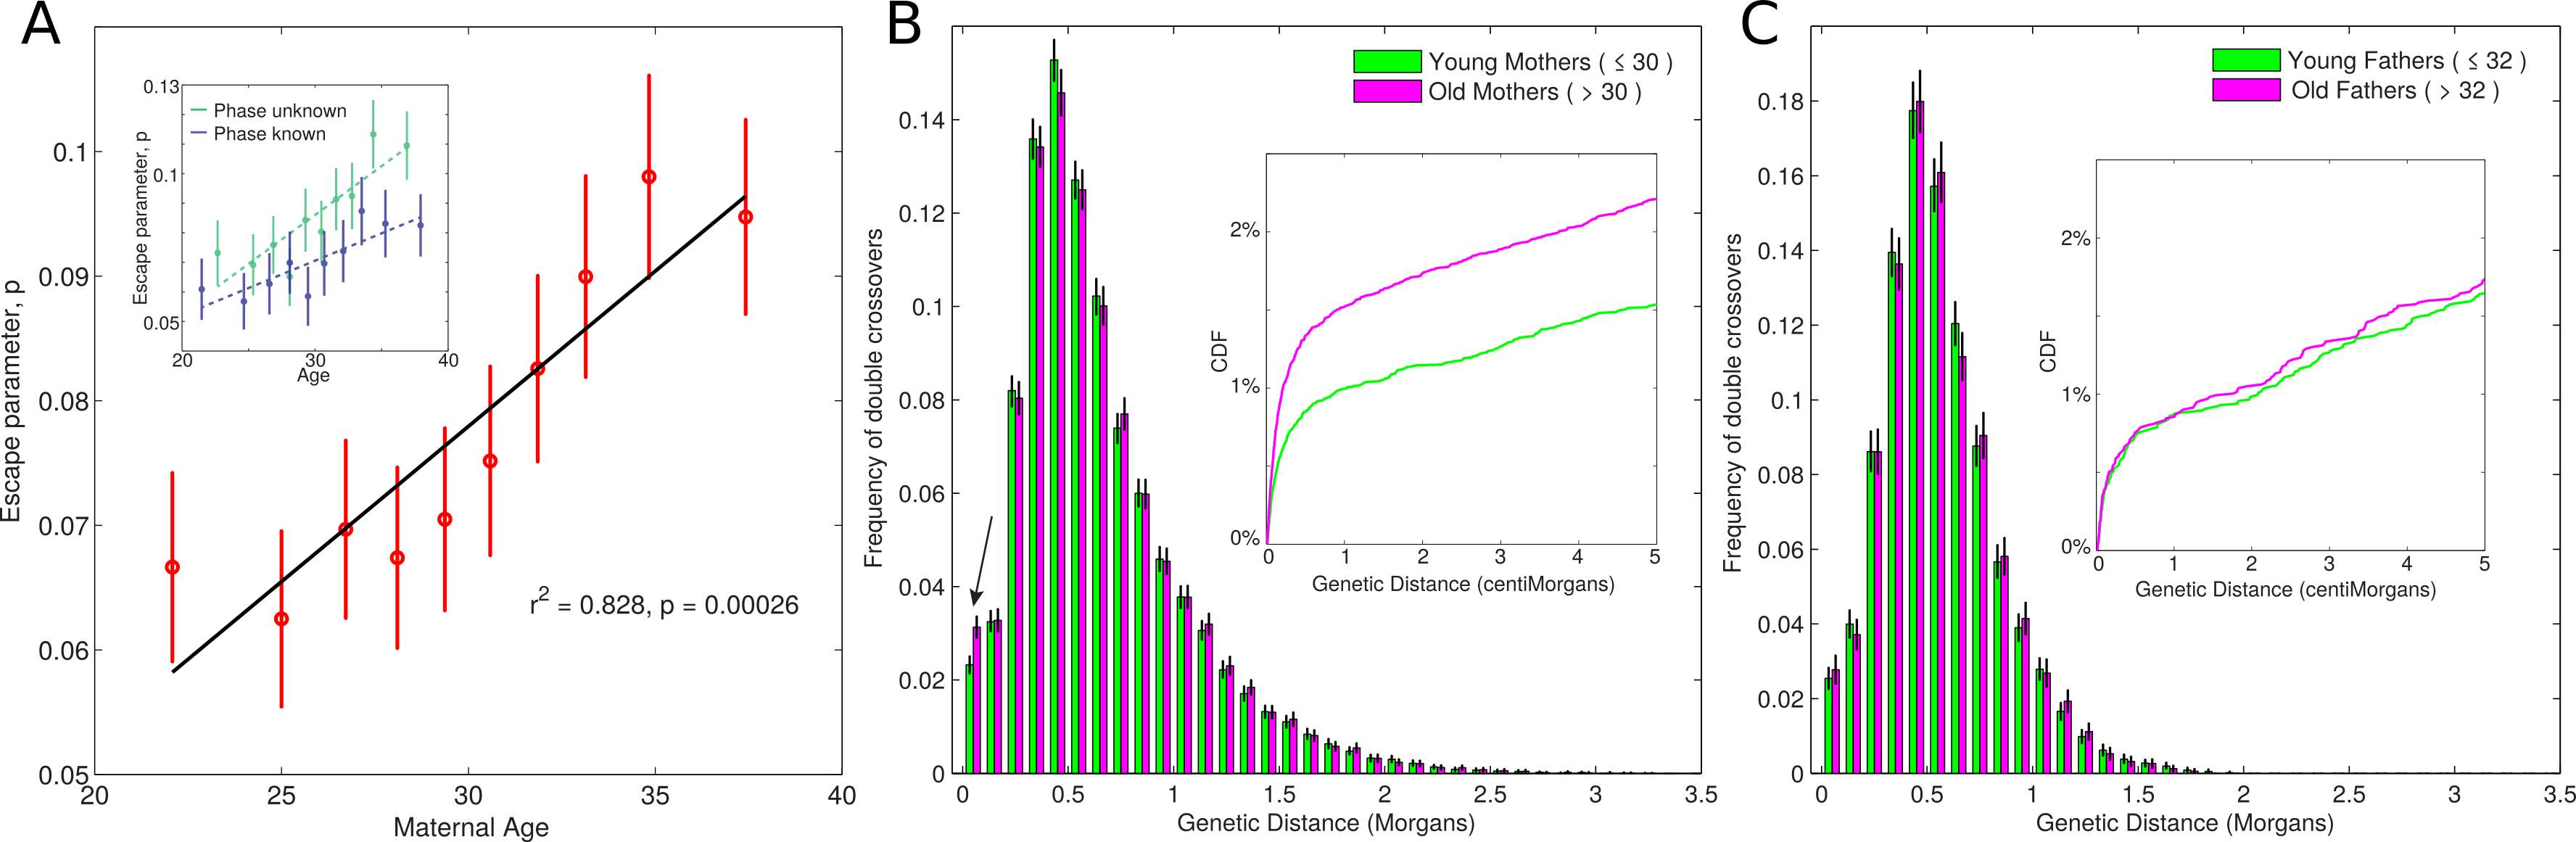
\includegraphics[width=\textwidth]{cointEscape/figs/Figure4.png}
    %\vspace{-20pt}
    \captionTitle{\textbf{Genetic map estimated from 23andMe data.}}{
        Genetic maps from the 23andMe data are shown in bold lines, whereas the genetic maps from deCODE are shown as thin lines.
        Separate maps are shown for females (red), males(blue), and sex-averaged (black).
        Also shown are regions highlighted in grey that represent gaps in the reference assembly. 
        For PAR1, we are showing data derived from Duffy\cite{Duffy2006} for comparison.
        As the deCODE maps cover a slightly smaller physical region than the 23andMe maps, the deCODE maps have been shifted slightly upwards to aid visual comparison.
        Specifically, the deCODE map has been aligned with the 23andMe map at the first physical position within the deCODE map.
        The locations of the alignments are indicated by small circles that can be most clearly seen on the smaller chromosomes.  
       \label{fig:cointFS4}}
\end{figure}

\begin{figure}[!h]
    %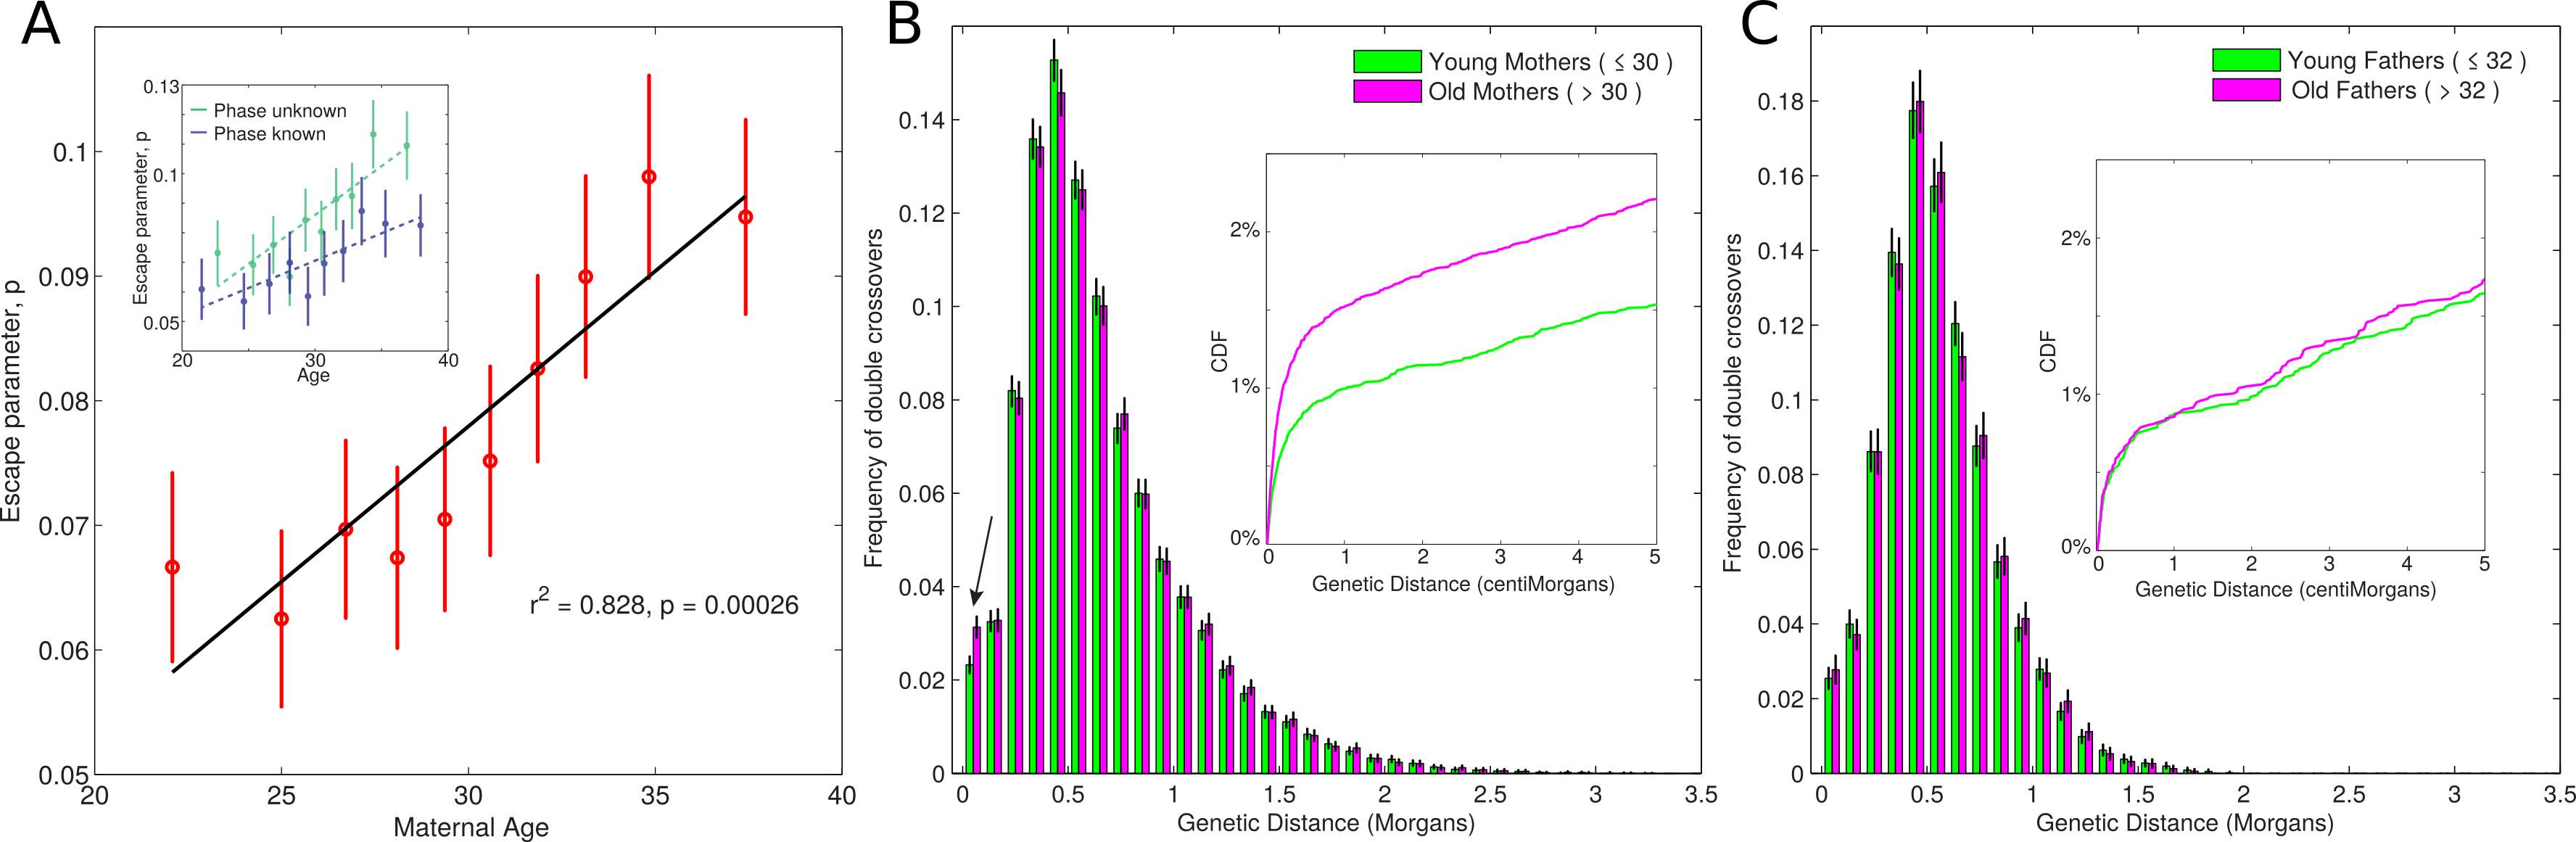
\includegraphics[width=\textwidth]{cointEscape/figs/Figure4.png}
    %\vspace{-20pt}
    \captionTitle{\textbf{The relationship between chromosome length and recombination.}}{ 
        The top row shows the correlation between physical length and map length for females (left), males (center), and sex averaged (right), with a linear fit included for the 23andMe map (red) and the deCODE map (blue).
        The bottom row shows the relationship between physical length and average recombination rate with a quadratic fit. 
        Note that chromosome X has been included in the female plots, but was excluded from the regressions.  
       \label{fig:cointFS5}}
\end{figure}

\begin{figure}[!h]
    %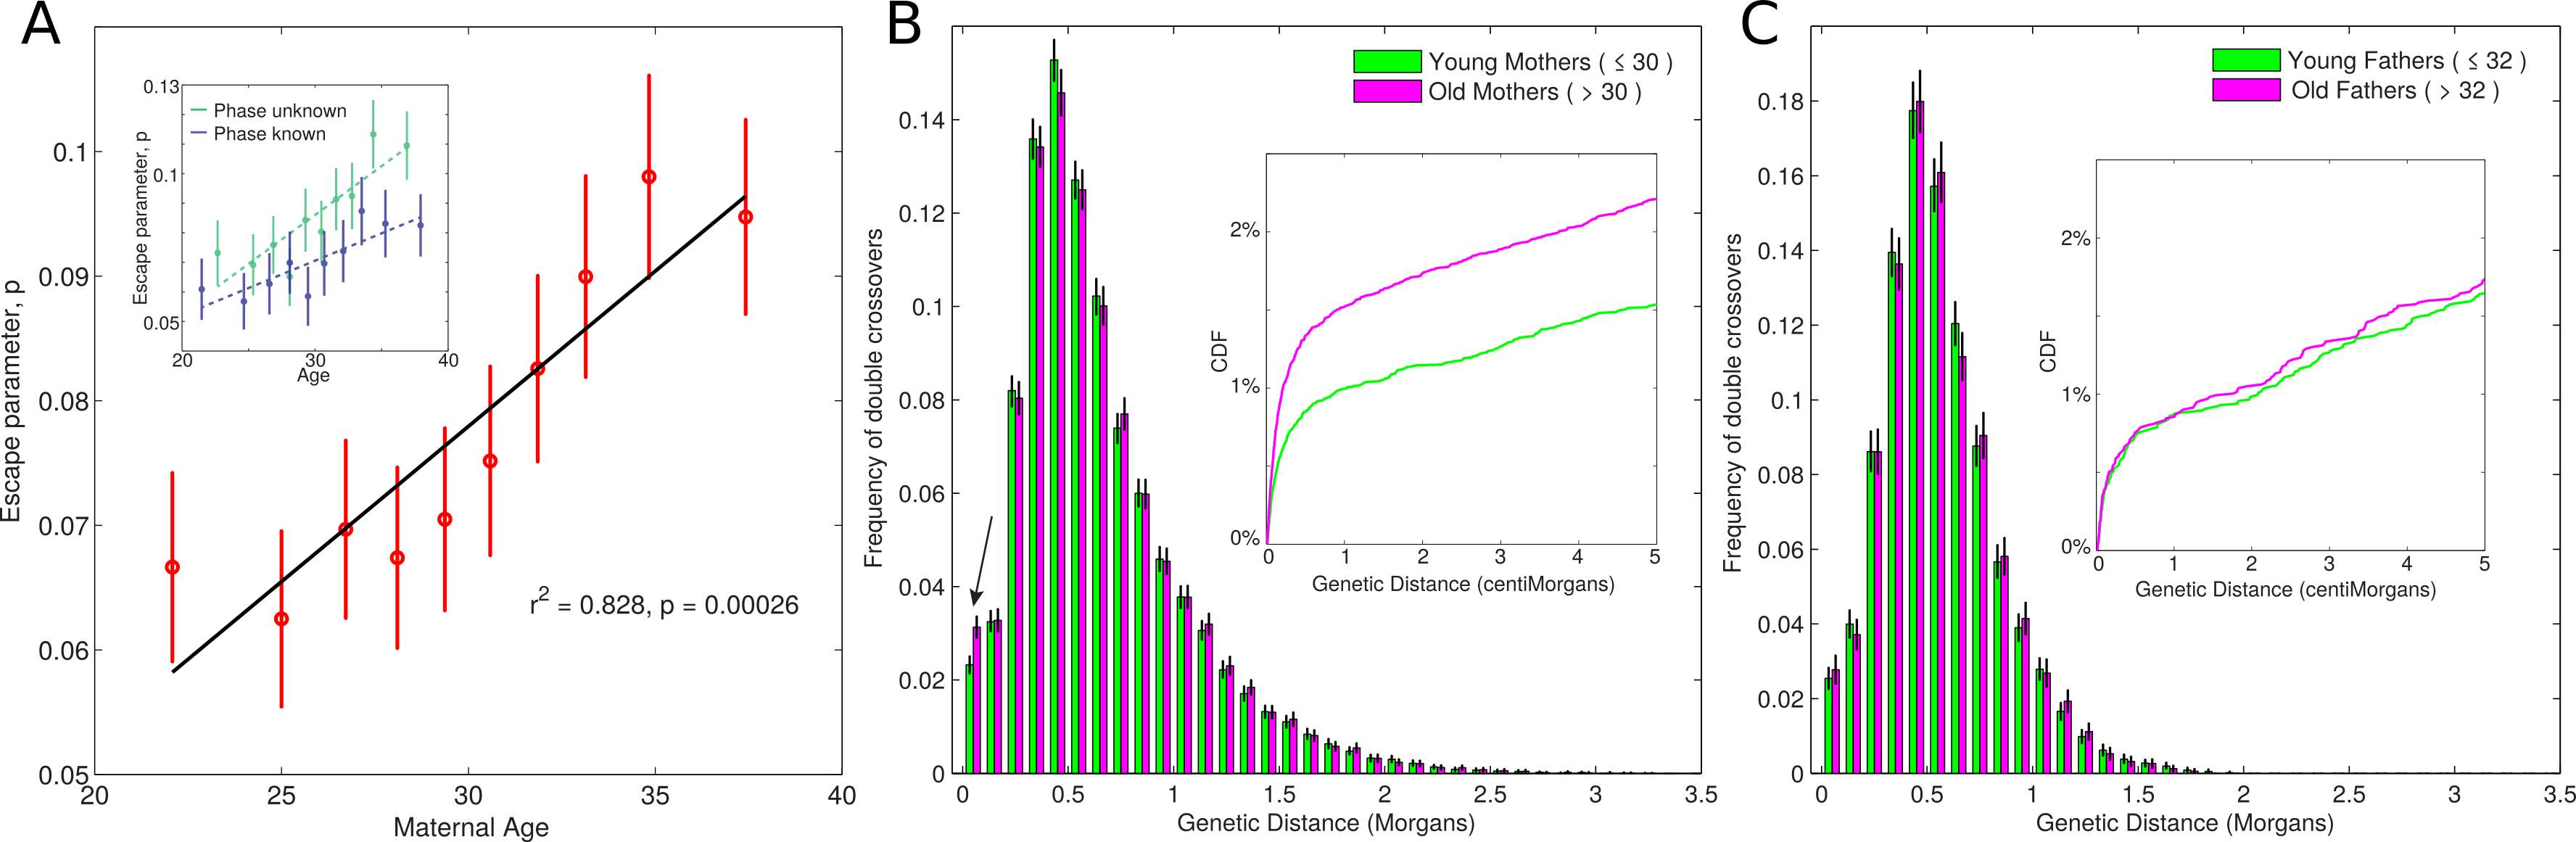
\includegraphics[width=\textwidth]{cointEscape/figs/Figure4.png}
    %\vspace{-20pt}
    \captionTitle{\textbf{Number of autosome recombination events verses parental age}}{
        for females (left) and males (right). 
        A linear least-squares fit is indicated by a black line.
        The least-squares fit equation given in the legend together with a p-value for the non-constant term.   
       \label{fig:cointFS6}}
\end{figure}

\begin{figure}[!h]
    %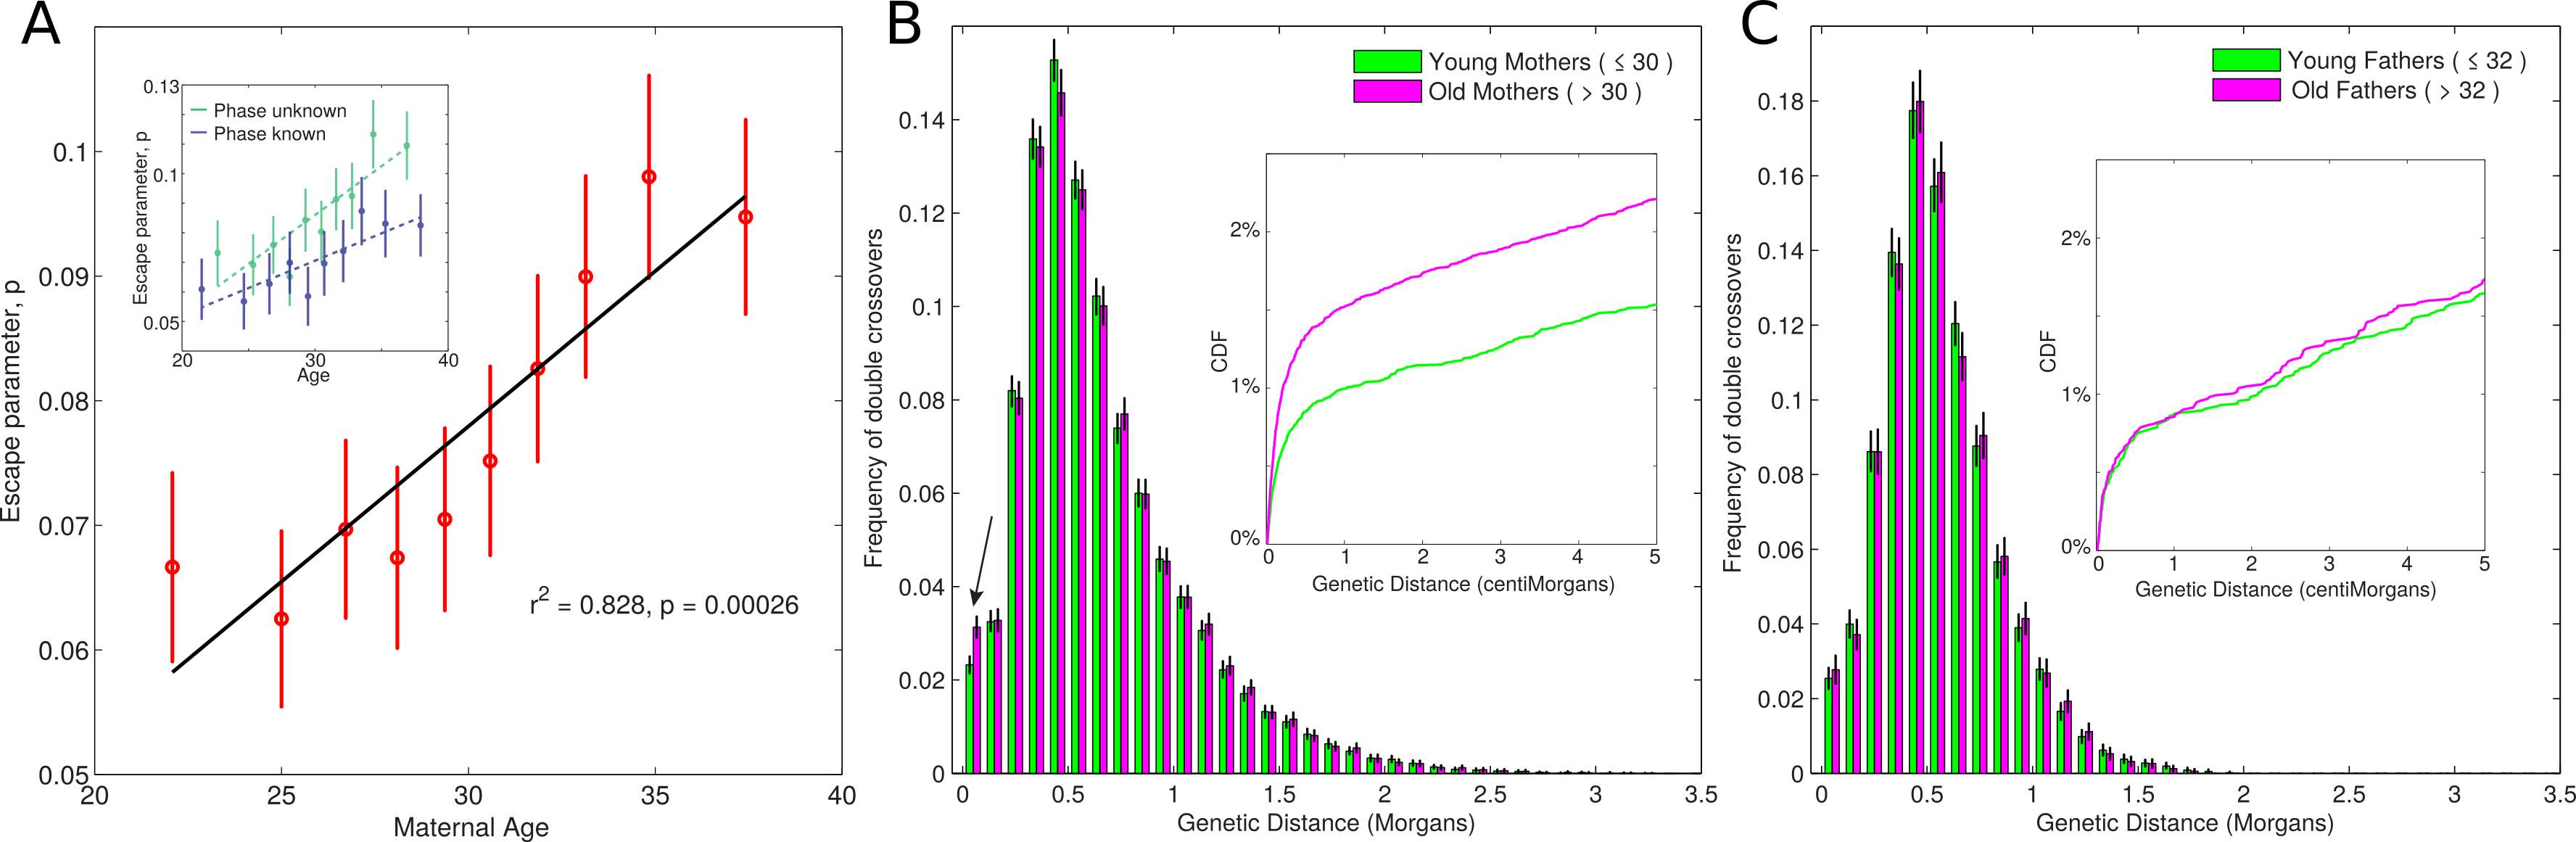
\includegraphics[width=\textwidth]{cointEscape/figs/Figure4.png}
    %\vspace{-20pt}
    \caption[\textbf{Hotspot usage between sexes.}]{
        A) Hotspot usage estimated in females (left) and males(right). 
        The MLE estimate for each individual is indicated by a circle, with a 95\% confidence interval indicated by the shaded area.
        The median MLE estimate for each sex is indicated by a vertical black line.
        B) Hotspot usage by parental age for females(left) and males (right).
        For each plot a logistic regression is also shown, with the p-value for the non-constant term given in the title.  
       \label{fig:cointFS7}}
\end{figure}

\begin{figure}[!h]
    %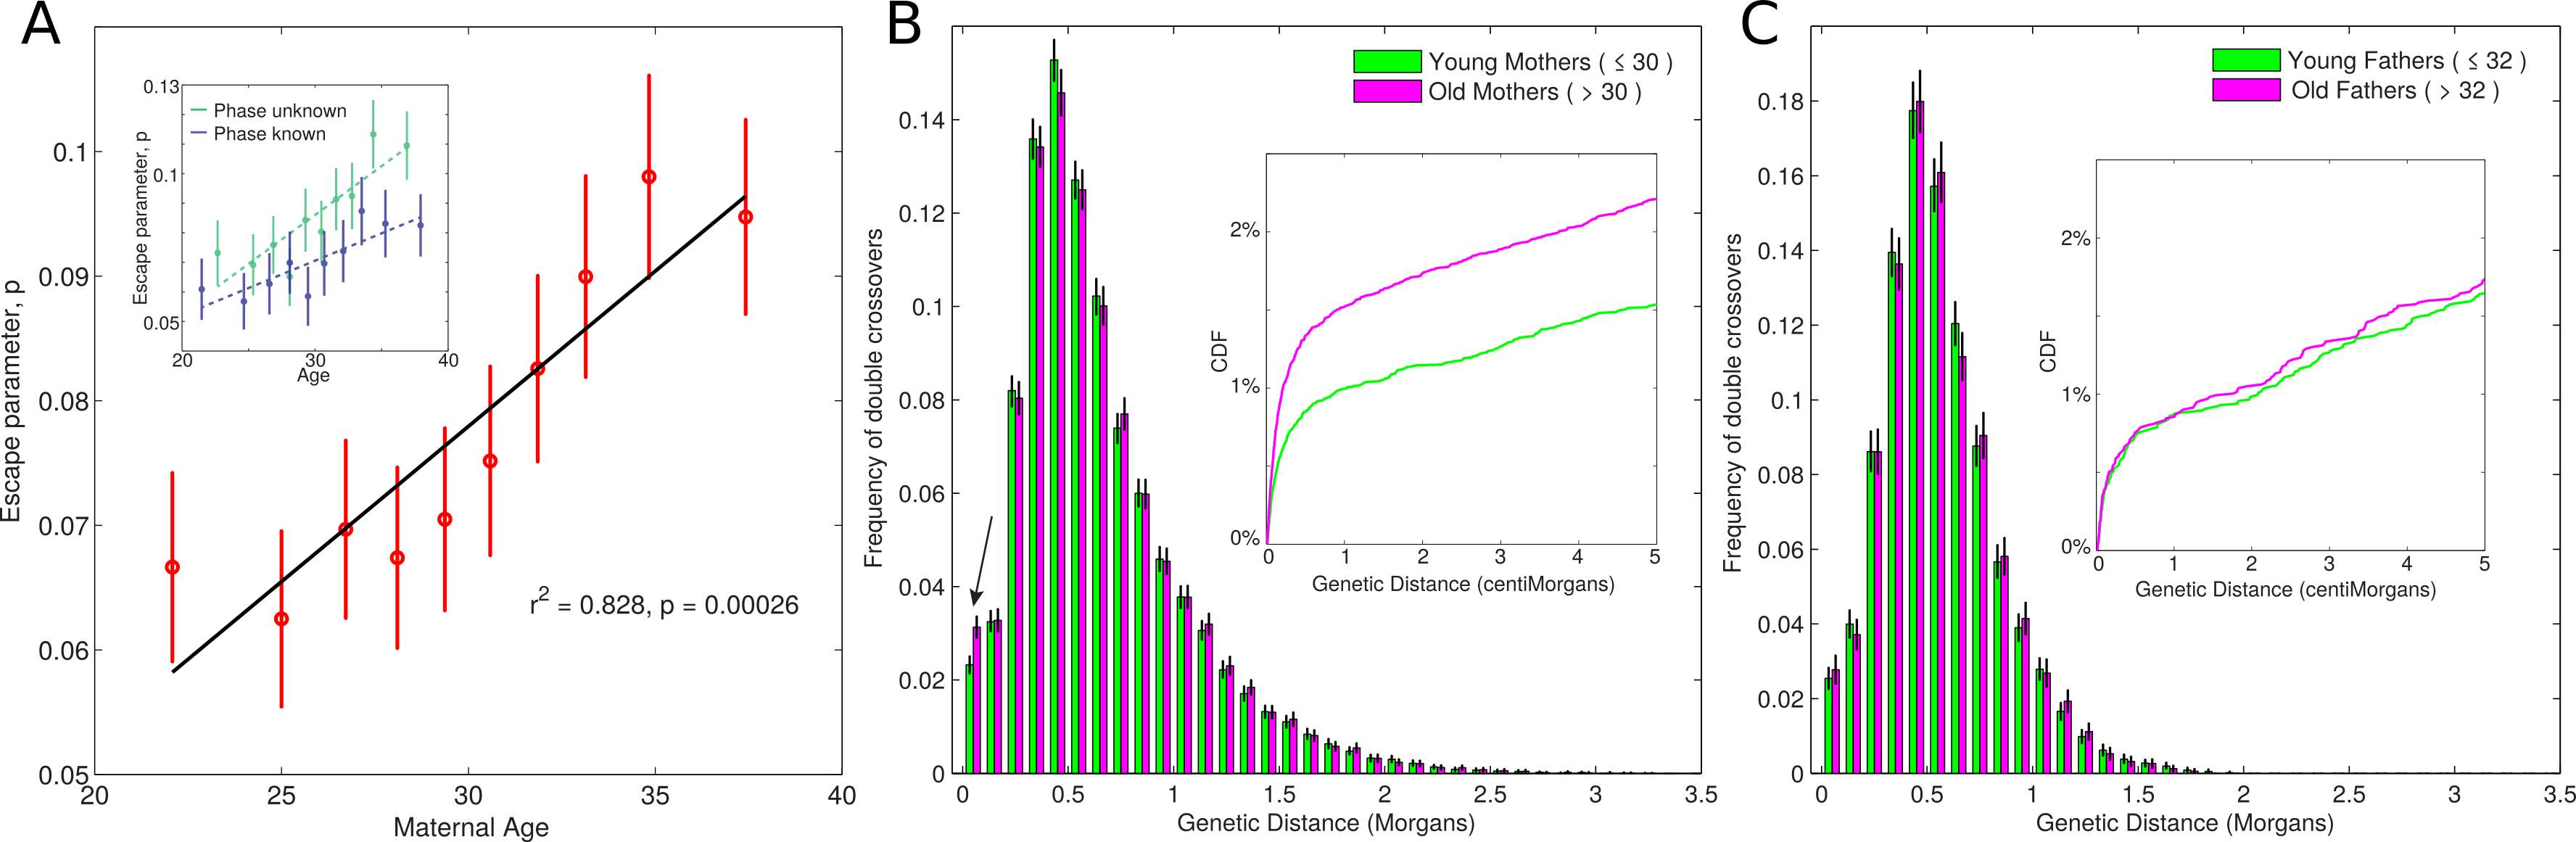
\includegraphics[width=\textwidth]{cointEscape/figs/Figure4.png}
    %\vspace{-20pt}
    \caption[\textbf{The relationship between map length and interference parameters.}]{ 
        A) The relationship between chromosome map length and the interference parameter, $\nu$.
        B) The relationship between chromosome map length and the escape parameter, $p$.
        Linear fits are shown for females (red), males (blue), and the data combined across sexes (black).
        In both plots, the chr21 estimate in males has been excluded.  
       \label{fig:cointFS8}}
\end{figure}

\begin{figure}[!h]
    %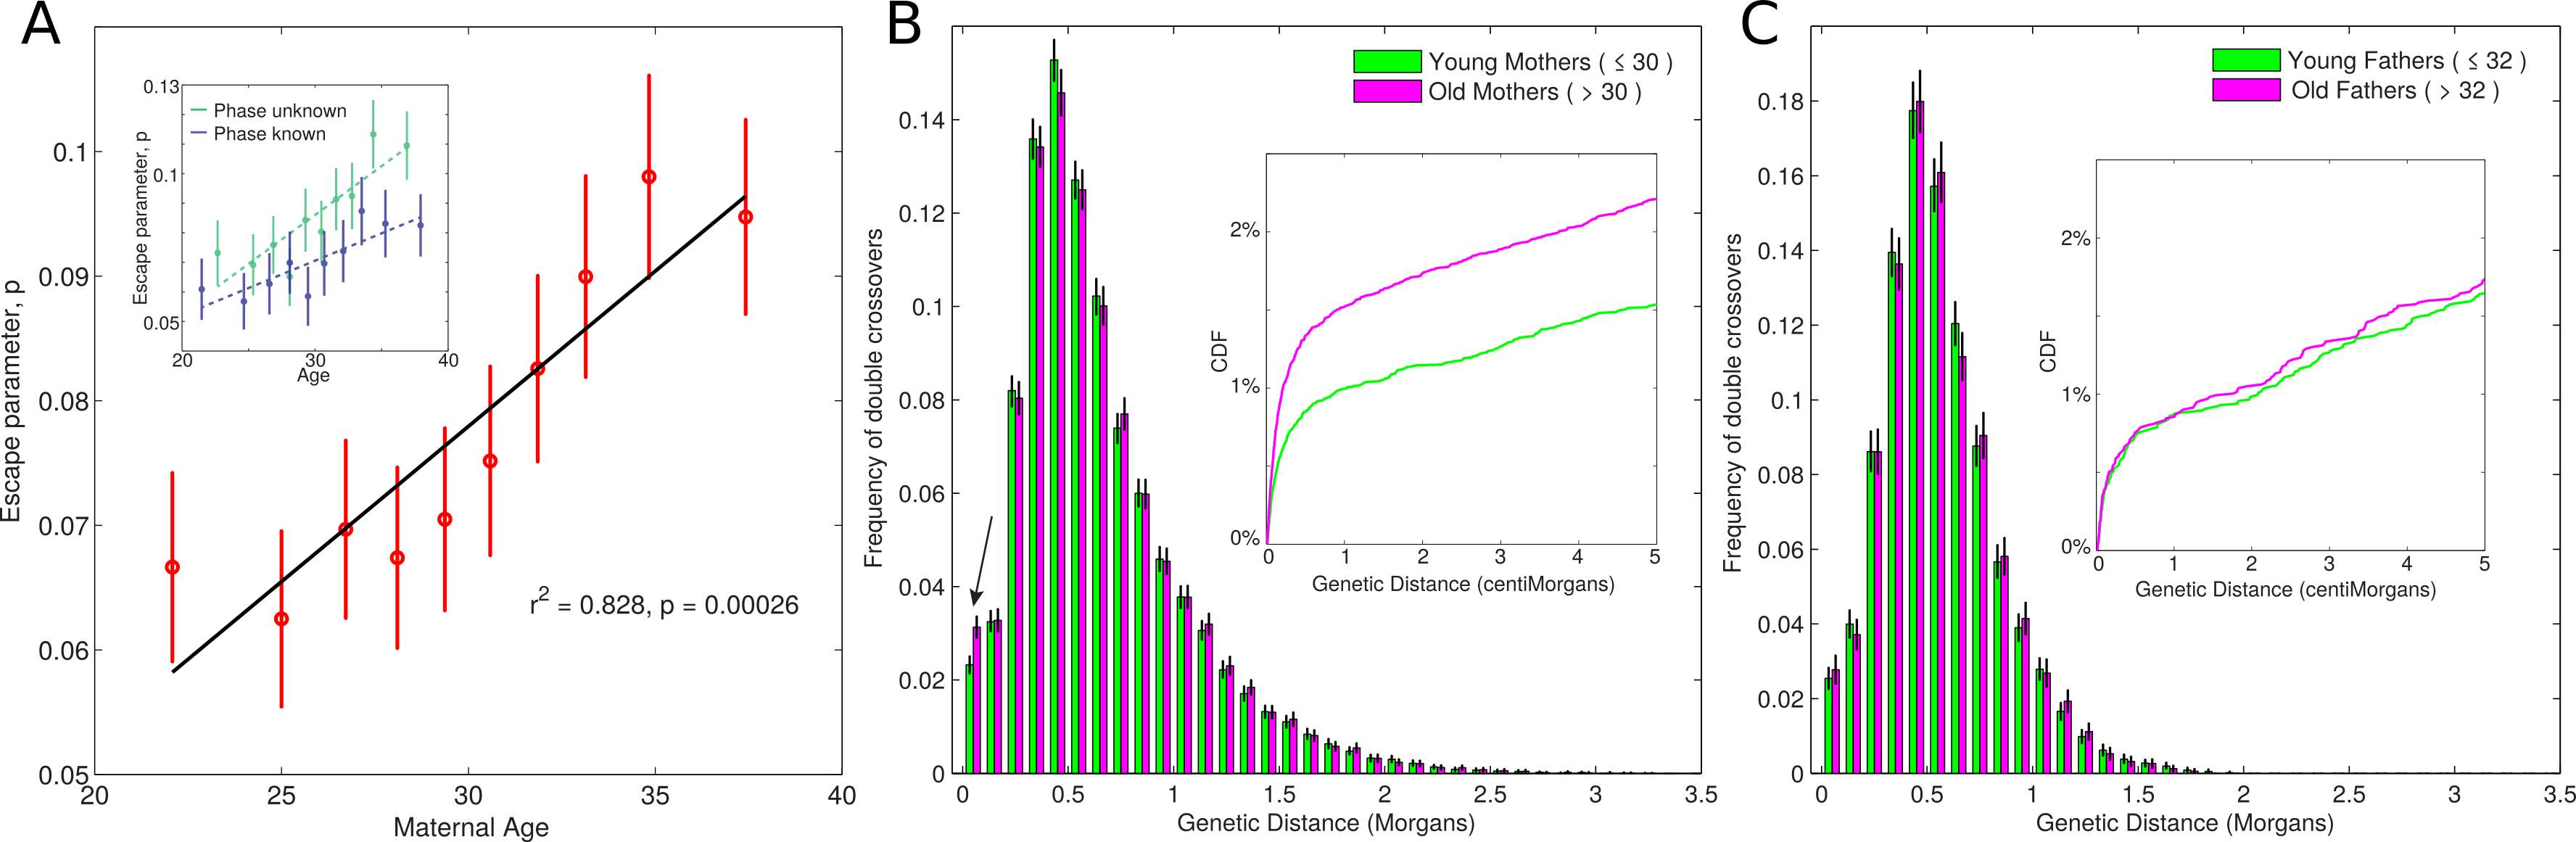
\includegraphics[width=\textwidth]{cointEscape/figs/Figure4.png}
    %\vspace{-20pt}
    \captionTitle{\textbf{Interference parameters as a function of age.}}{
        Females and males are shown on the top and bottom rows respectively. 
        Estimates of the interference parameter, $\nu$, are shown on the left, whereas estimates of the escape parameter, $p$, are shown on the right.
        Error bars show 95\% confidence intervals.  
       \label{fig:cointFS9}}
\end{figure}

\begin{figure}[!h]
    %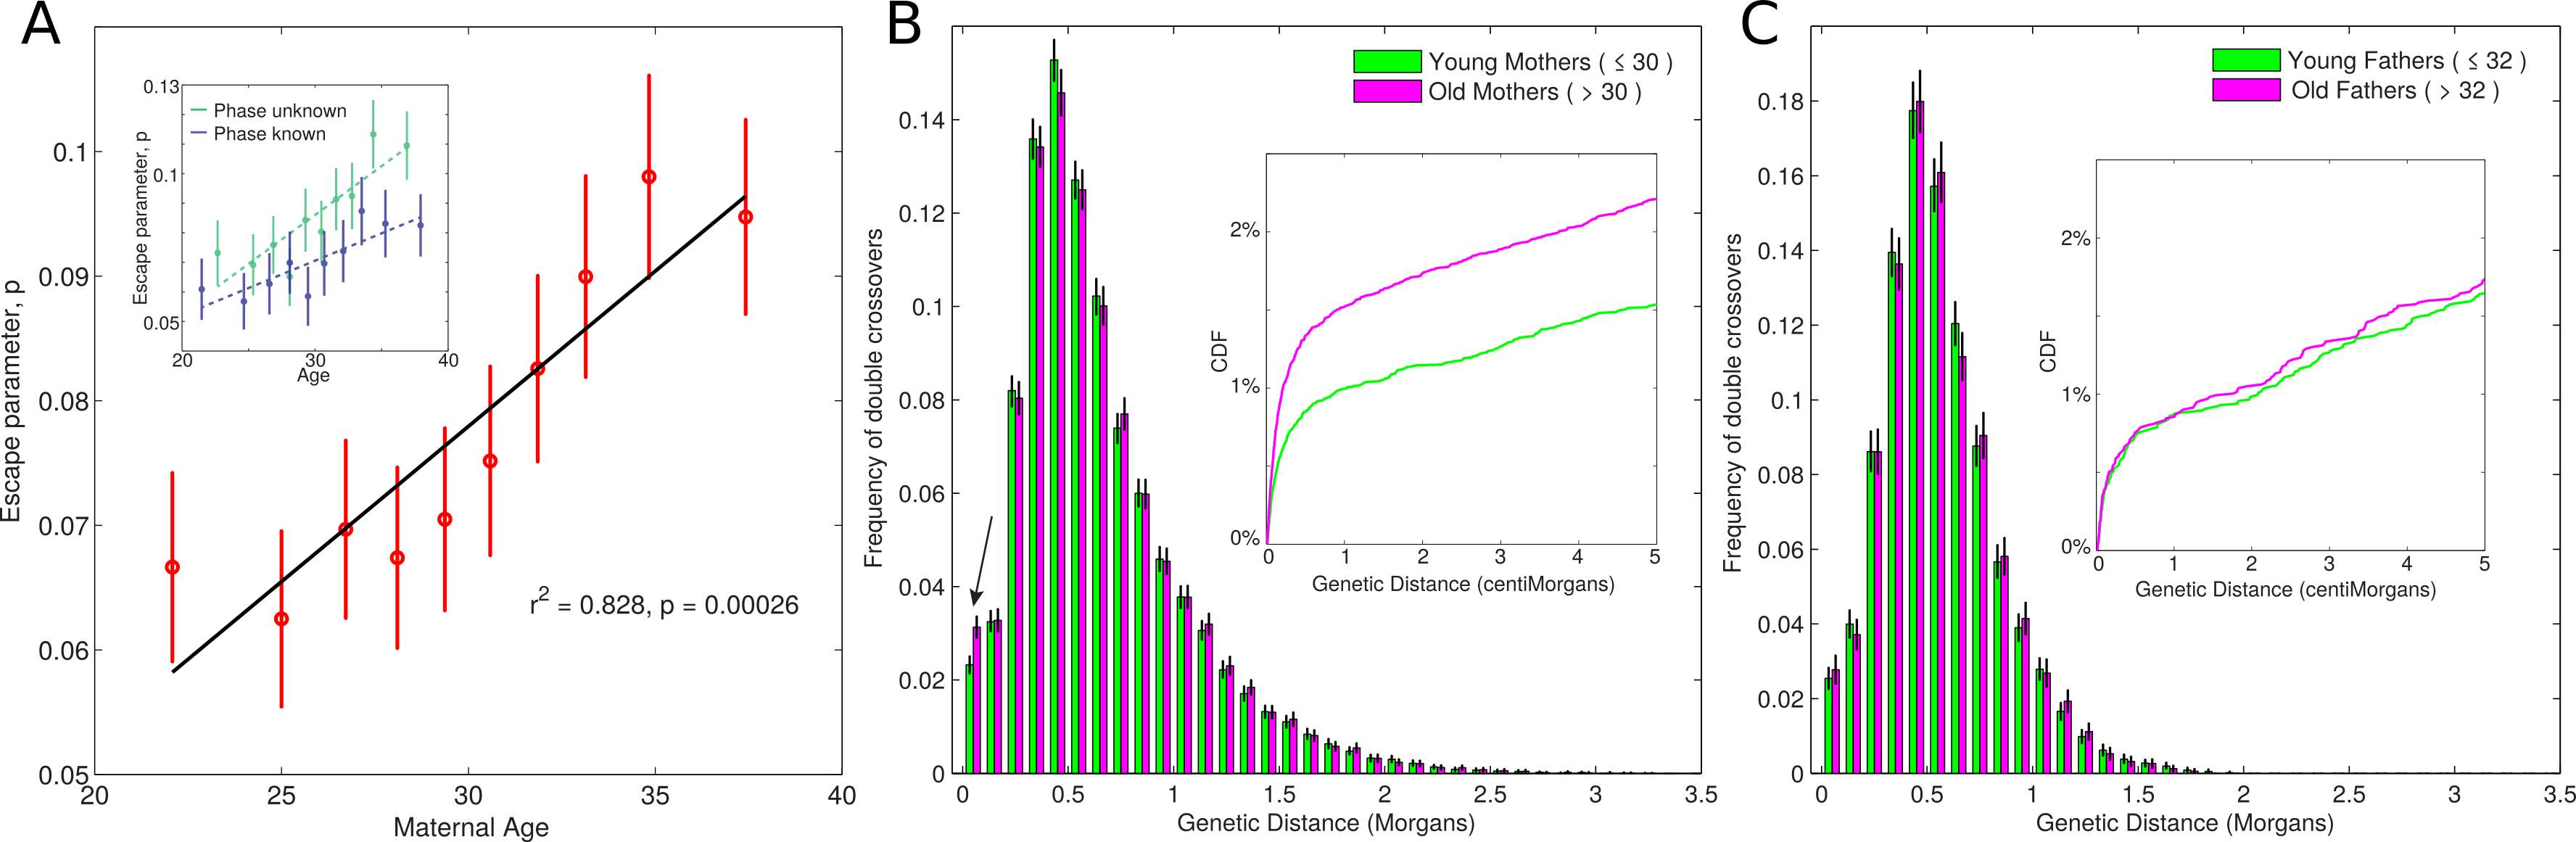
\includegraphics[width=\textwidth]{cointEscape/figs/Figure4.png}
    %\vspace{-20pt}
    \captionTitle{\textbf{Interference parameters by age}}{,
        having divided the data in 5 or 20 age quantiles.
        Error bars show 95\% confidence intervals.  
       \label{fig:cointFS10}}
\end{figure}

\begin{figure}[!h]
    %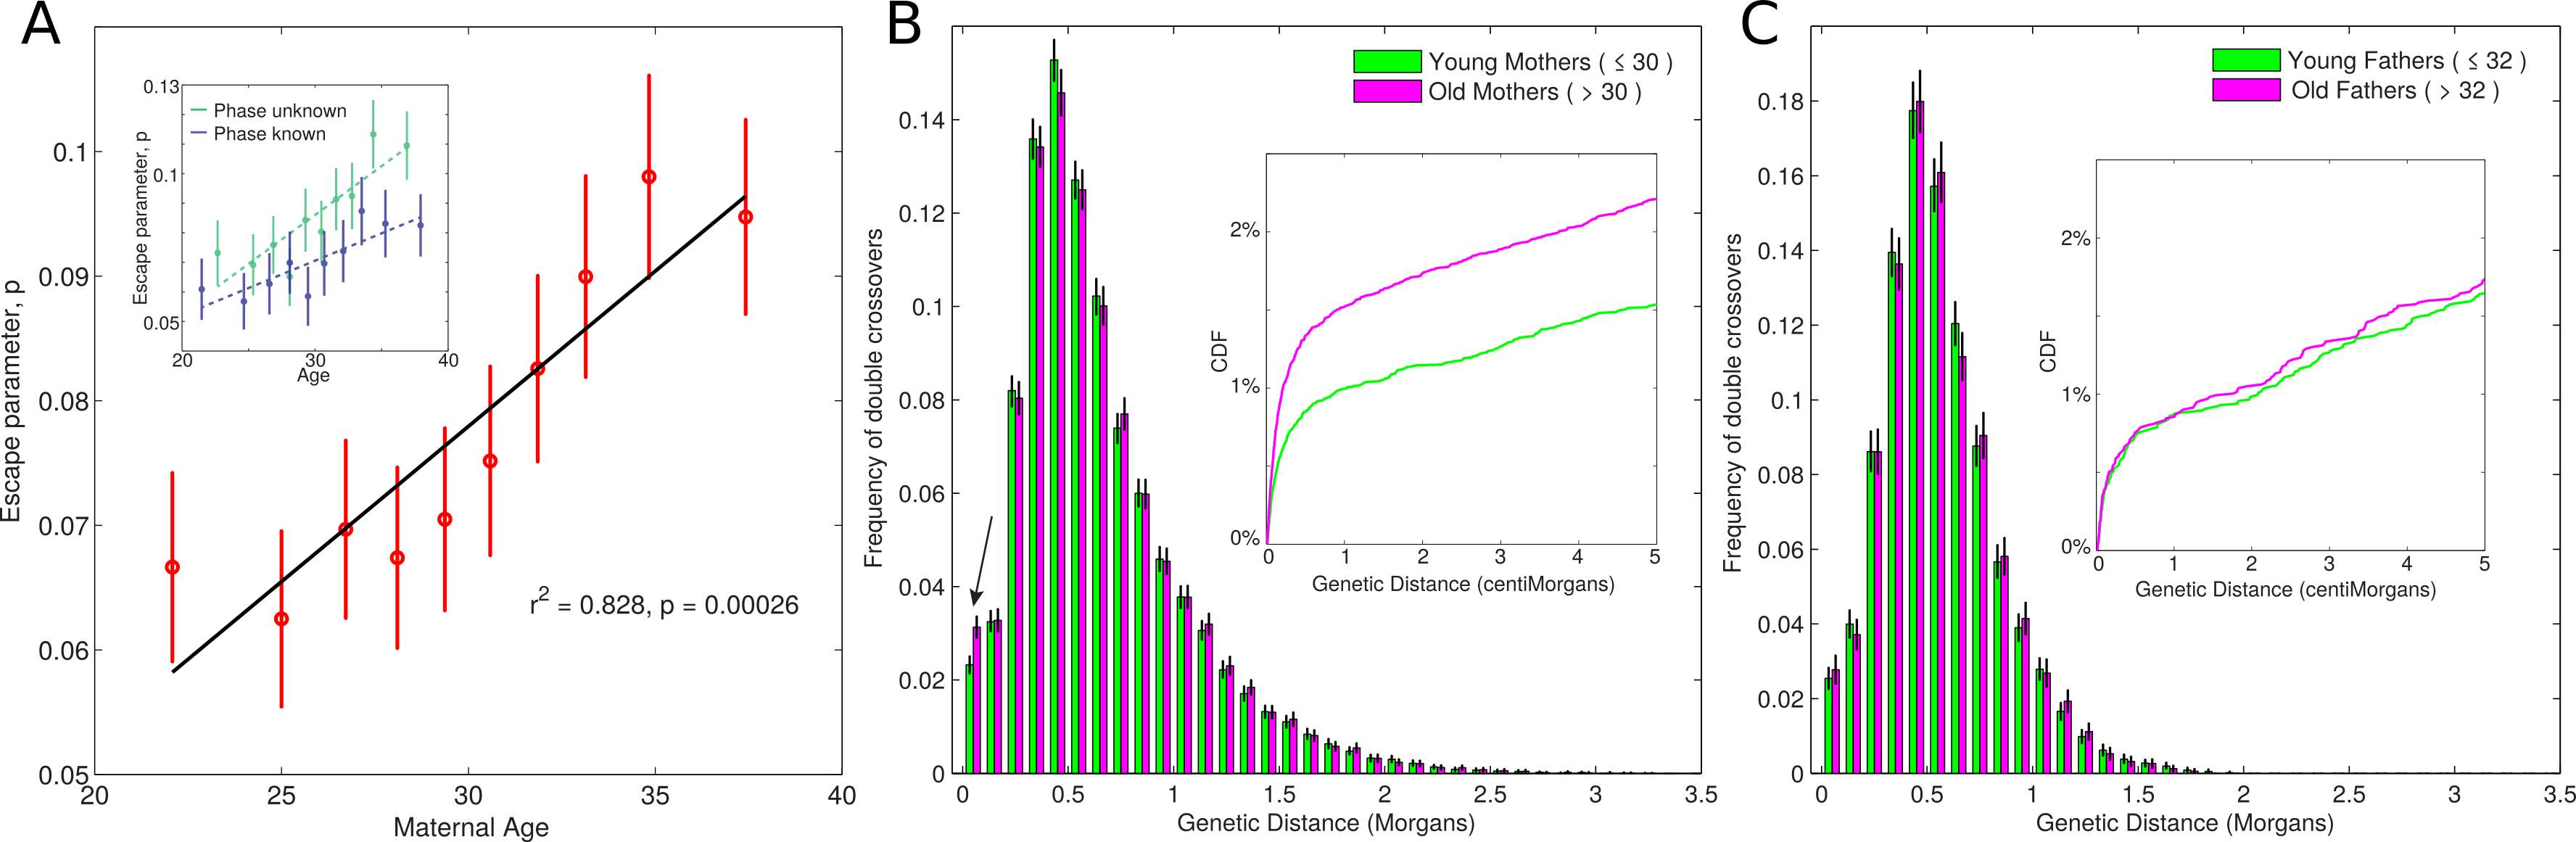
\includegraphics[width=\textwidth]{cointEscape/figs/Figure4.png}
    %\vspace{-20pt}
    \caption{\textbf{Interference parameters by age and phase.}}{ 
        Interference parameters by age, having estimated the interference parameters for phase-known and phase-unknown groups separately.  
       \label{fig:cointFS11}}
\end{figure}

\begin{figure}[!h]
    %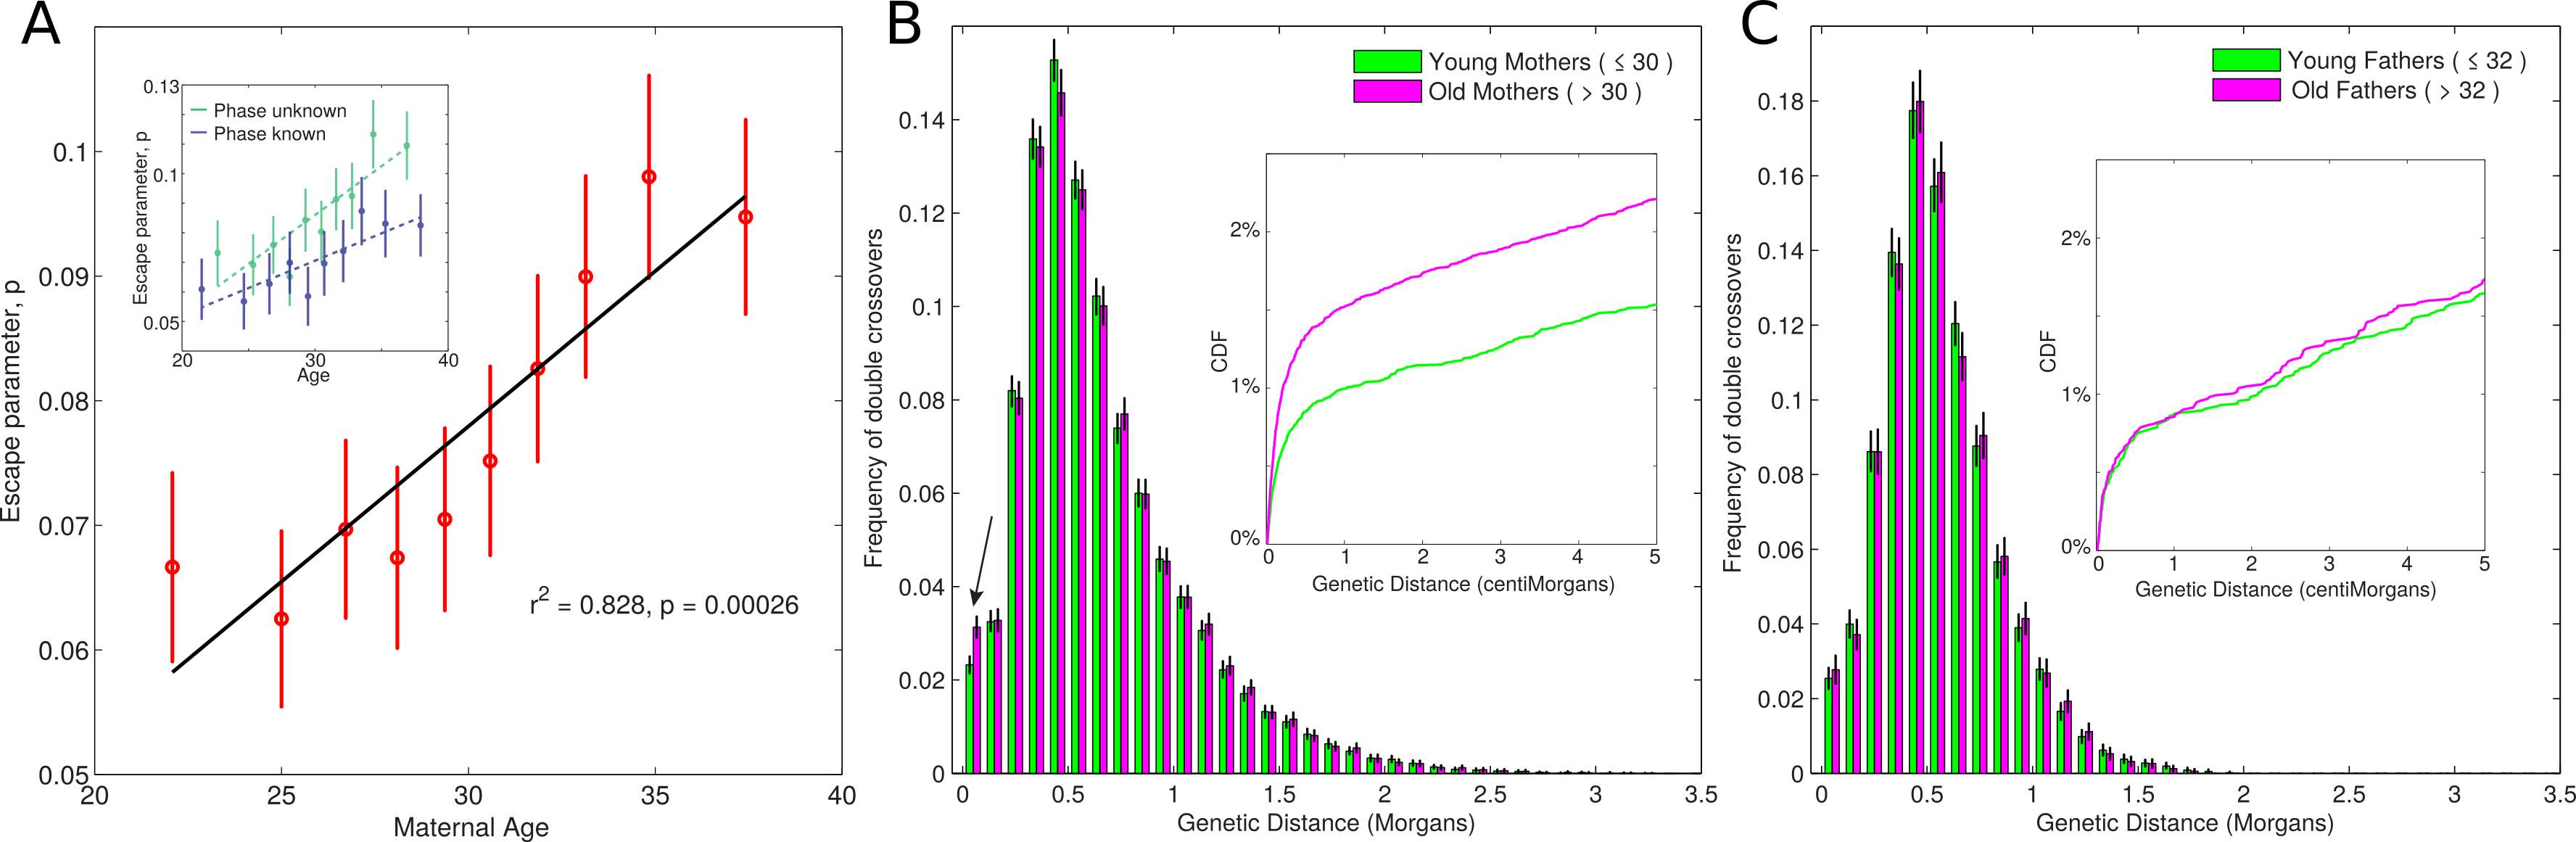
\includegraphics[width=\textwidth]{cointEscape/figs/Figure4.png}
    %\vspace{-20pt}
    \captionTitle{\textbf{Interference parameters as a function of age, following stratified sampling.}}{
        Females and males are shown on the top and bottom rows respectively.
        Estimates of the interference parameter, $\nu$, are shown on the left, whereas estimates of the escape parameter, $p$, are shown on the right.
        Error bars show 95\% confidence intervals.  
       \label{fig:cointFS12}}
\end{figure}

\begin{figure}[!h]
    %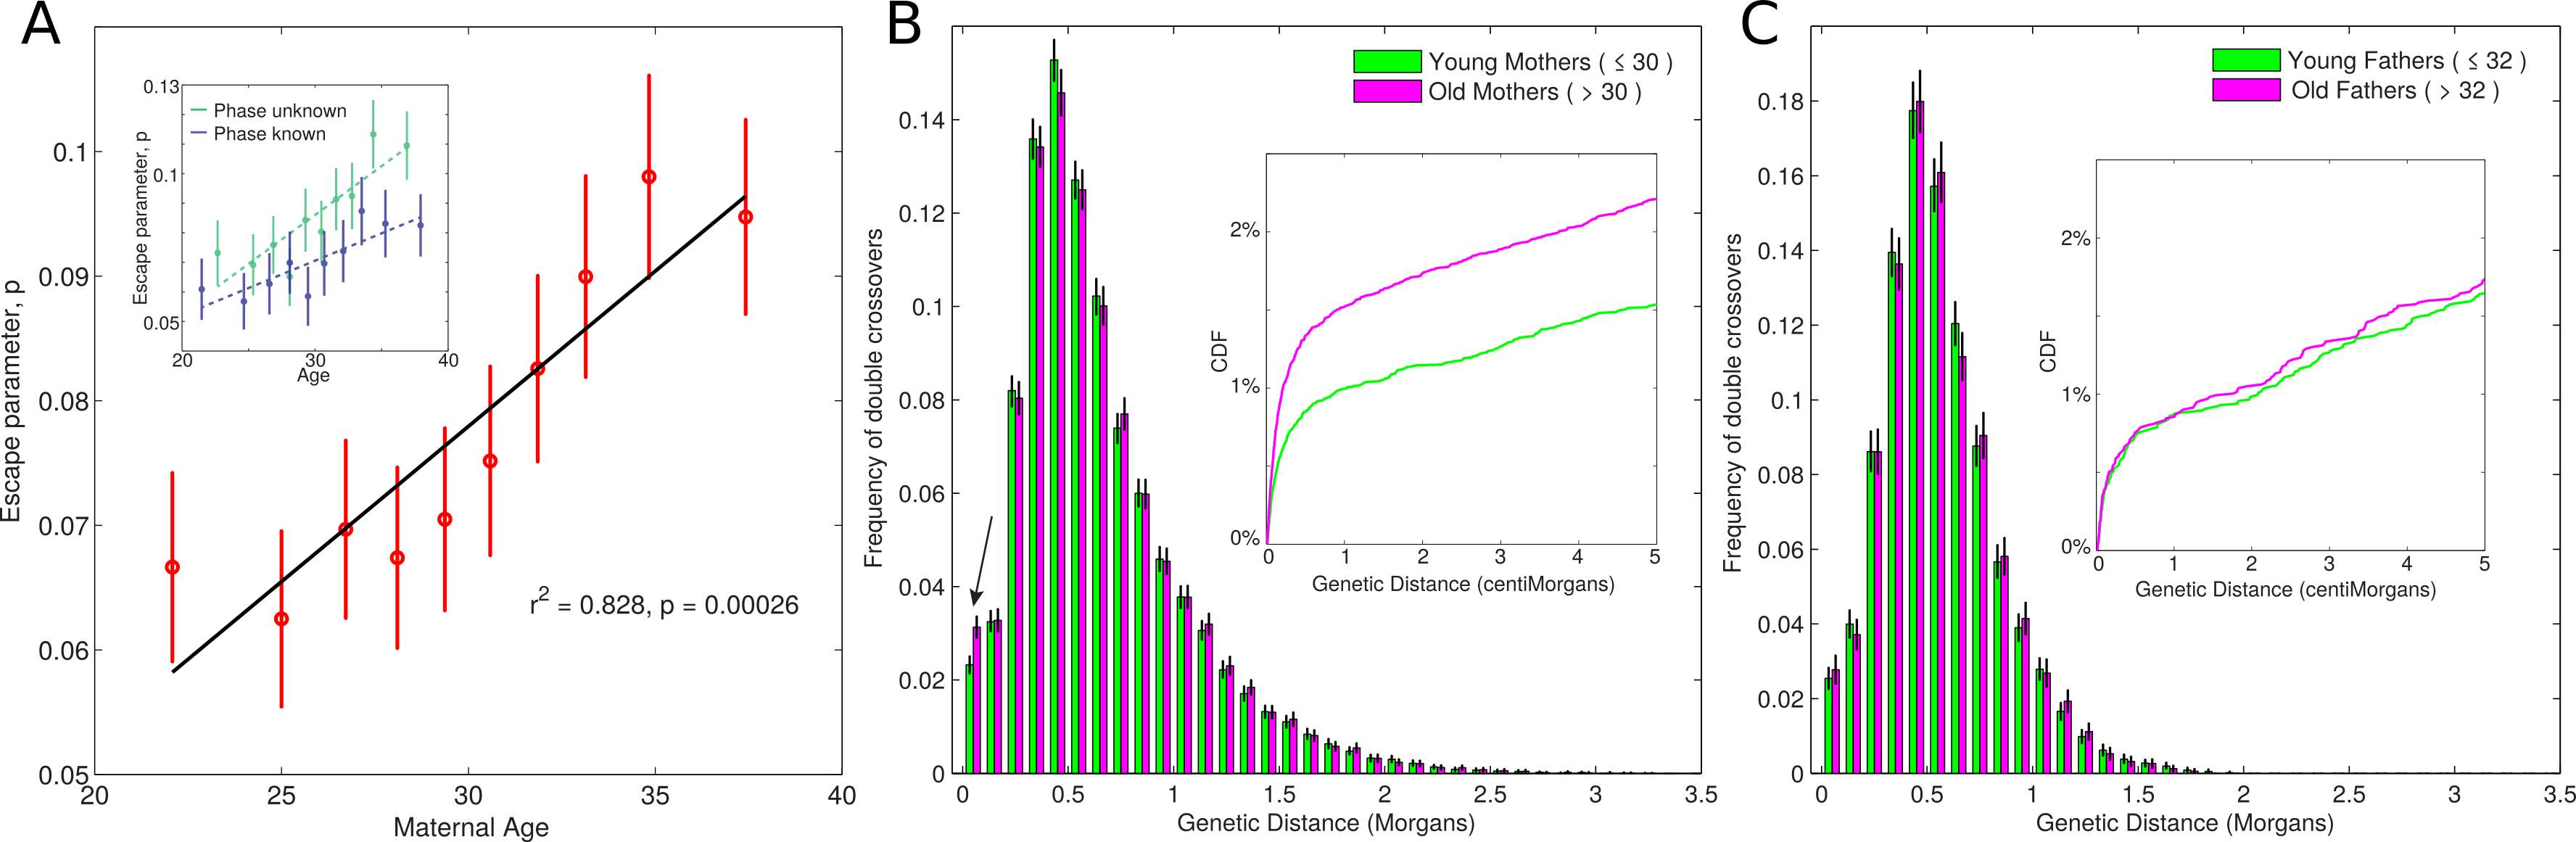
\includegraphics[width=\textwidth]{cointEscape/figs/Figure4.png}
    \vspace{-20pt}
    \captionTitle{\textbf{Model fit for tightly clustered events}}{
        in females (A) and males (B).
        The figure shows the empirical cumulative distribution function for young (green line) and old (magenta line) mothers/fathers, and compares to that obtained via simulation under the interference free model (black dotted line), the Gamma simple interference model (black dashed line), and the Housworth-Stahl interference escape model (solid black line), with parameters were taken from Supplementary Table 7.
        The figure is shown on a log-log scale to emphasize the short inter-crossover distances.  
       \label{fig:cointFS13}}
\end{figure}

\begin{figure}[!h]
    %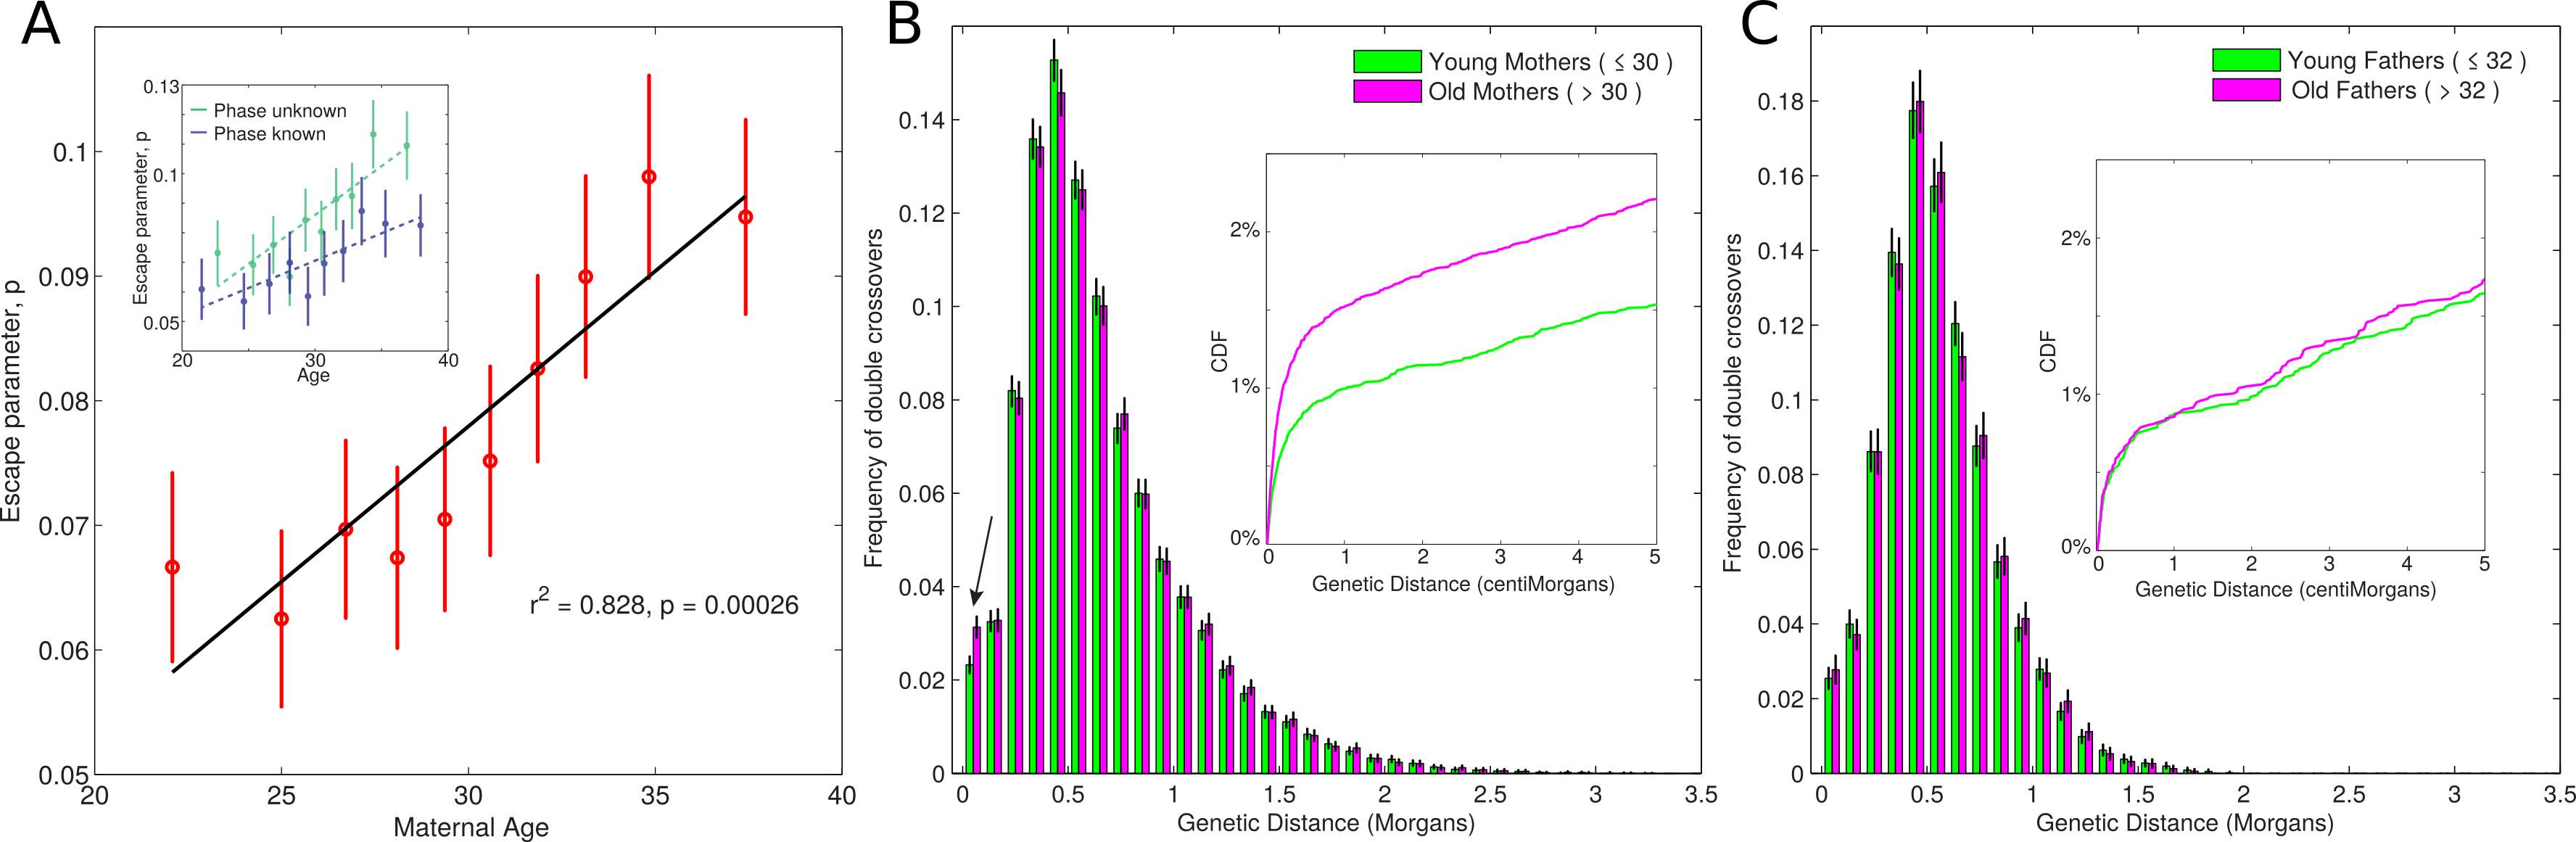
\includegraphics[width=\textwidth]{cointEscape/figs/Figure4.png}
    \vspace{-20pt}
    \captionTitle{\textbf{Interference parameters estimated for a strictly filtered dataset.}}{
        In this case, all crossover events were required at least 10 supporting informative sites (compared to 3 in the main dataset), no two events within a single family were allowed to be within 5 SNPs of each other (compared to 1 in the main dataset), and no more than 4 events within 1 Mb of each other were allowed across the whole dataset (and compared to 14 in the main dataset, which corresponds to the 99.9\textsuperscript{th} percentile).
        After this very strict filtering, the deviation from the Housworth-Stahl interference escape model is much less pronounced at short scales (right hand panels), but the association between interference escape and maternal  
        age remains strong (2\textsuperscript{nd} panel from top left).   
       \label{fig:cointFS14}}
\end{figure}


\subsection{Supplementary Tables}


\begin{table}[!h] \centering
    \begin{tabular}{|c|c|c|c|} 
        \hline Pedigree Type & Description & Before Filtering & After Filtering \\ \hline
        1 & 2 parents, 2 children & 3319 & 3307 \\
        2 & 2 parents, 3 children & 560 & 523 \\
        3 & 2 parents, 4 children & 89 & 80 \\
        4 & Quartet, with 2nd generation trio & 101 & 100 \\
        5 & Trio, with 2nd generation quartet & 201 & 199 \\
        \hline & \textbf{Total} & \textbf{4270} & \textbf{4209} \\
    \hline \end{tabular}
    \captionTitle{\textbf{Summary of dataset, before and after filtering.}}{
    \label{tab:cointTS1}}
\end{table}

\begin{table}[!h] \centering
    \begin{tabular}{|p{3cm}p{1.5cm}p{1.5cm}p{1.5cm}p{1.5cm}p{1.5cm}p{2cm}|}
        \hline 
    Population & Female \mbox{unphased} & Male \mbox{unphased} & Female phased & Male phased & Total Meioses & Percentage \\ \hline
    Europe & 5382 & 5508 & 1789 & 1641 & 14320 & 78.24\% \\
    Latino & 602 & 546 & 171 & 190 & 1509 & 8.25\% \\
    East Asia & 380 & 308 & 88 & 74 & 850 & 4.64\% \\
    None/Other & 198 & 268 & 68 & 109 & 643 & 3.51\% \\
    South Asia & 178 & 176 & 19 & 20 & 393 & 2.15\% \\
    African American & 152 & 152 & 34 & 36 & 374 & 2.04\% \\
    Middle East & 76 & 100 & 15 & 22 & 213 & 1.16\% \\
    \hline \textbf{Total} & \textbf{6968} & \textbf{7058} & \textbf{2184} & \textbf{2092} & \textbf{18302} & \textbf{100.00\%} \\
    \hline \end{tabular}
    \captionTitle{\textbf{Description of parental ancestry for each meiosis within the sample.}} {
    \label{tab:cointTS2}}
\end{table}

\begin{table}[!h] \centering
    \footnotesize
    \begin{tabular}{|cp{1.2cm}p{1.4cm}p{1.1cm}p{1.1cm}p{1.0cm}p{1.1cm}p{1.0cm}p{1.1cm}p{1.0cm}|}
        \hline 
Chrom & First Position (bp) & Last Position (bp) & Physical Length (Mb) & Female Map Length (cM) & Female Mean Rate (cM/Mb) & Male Map Length (cM) & Male Mean Rate (cM/Mb) & SexAvg Map Length (cM) & SexAvg Mean Rate (cM/Mb) \\ \hline
chr1 & 1,031,540 & 249,170,711 & 248.14 & 335.9 & 1.36 & 198.30 & 0.80 & 267.05 & 1.08 \\
chr2 & 118,913 & 242,763,542 & 242.64 & 316.45 & 1.31 & 184.64 & 0.76 & 250.52 & 1.03 \\
chr3 & 152,592 & 197,759,785 & 197.61 & 270.98 & 1.37 & 163.85 & 0.83 & 217.4 & 1.1 \\
chr4 & 167,596 & 190,787,660 & 190.62 & 260.11 & 1.37 & 145.79 & 0.76 & 202.93 & 1.06 \\
chr5 & 184,702 & 180,673,228 & 180.49 & 249.13 & 1.38 & 146.66 & 0.81 & 197.87 & 1.1 \\
chr6 & 188,937 & 170,777,087 & 170.59 & 236.64 & 1.39 & 140.88 & 0.83 & 188.74 & 1.11 \\
chr7 & 67,365 & 159,042,351 & 158.97 & 223.17 & 1.41 & 136.04 & 0.86 & 179.55 & 1.13 \\
chr8 & 200,898 & 146,235,564 & 146.03 & 210.94 & 1.45 & 122.41 & 0.84 & 166.64 & 1.14 \\
chr9 & 215,269 & 141,004,945 & 140.79 & 195.69 & 1.4 & 125.54 & 0.89 & 160.58 & 1.14 \\
chr10 & 162,102 & 135,402,200 & 135.24 & 207.86 & 1.54 & 129.91 & 0.96 & 168.86 & 1.25 \\
chr11 & 244,552 & 134,872,342 & 134.63 & 193.59 & 1.44 & 120.21 & 0.89 & 156.88 & 1.17 \\
chr12 & 216,039 & 133,684,321 & 133.47 & 200.36 & 1.51 & 131.20 & 0.98 & 165.75 & 1.24 \\
chr13 & 19,458,371 & 114,998,076 & 95.54 & 152.26 & 1.6 & 101.19 & 1.06 & 126.71 & 1.33 \\
chr14 & 20,445,905 & 107,233,999 & 86.79 & 137.22 & 1.59 & 97.29 & 1.12 & 117.24 & 1.35 \\
chr15 & 22,763,396 & 102,381,360 & 79.62 & 143.39 & 1.8 & 100.85 & 1.27 & 122.11 & 1.53 \\
chr16 & 143,503 & 90,102,384 & 89.96 & 157.29 & 1.75 & 102.03 & 1.13 & 129.64 & 1.44 \\
chr17 & 84,782 & 81,025,393 & 80.94 & 152.87 & 1.9 & 106.23 & 1.31 & 129.53 & 1.6 \\
chr18 & 218,695 & 77,955,378 & 77.74 & 140.06 & 1.81 & 97.80 & 1.26 & 118.91 & 1.53 \\
chr19 & 288,246 & 59,058,083 & 58.77 & 117.8 & 2.01 & 99.42 & 1.69 & 108.59 & 1.85 \\
chr20 & 100,699 & 62,892,739 & 62.79 & 118.9 & 1.9 & 99.00 & 1.58 & 108.93 & 1.73 \\
chr21 & 14,807,136 & 47,978,421 & 33.17 & 74.34 & 2.24 & 51.76 & 1.58 & 63.04 & 1.9 \\
chr22 & 17,152,611 & 51,165,664 & 34.01 & 78.16 & 2.31 & 63.30 & 1.86 & 70.71 & 2.08 \\
chrX & 2,737,282 & 154,408,041 & 151.67 & 179.02 & 1.18 &  &  &  &  \\
PAR1 & 178,624 & 2,689,575 & 2.51 & 2.73 & 1.16 & 42.94 & 17.17 & 22.75 & 9.06 \\
PAR2 & 154,984,651 & 155,227,607 & 0.24 & 0.05 & 0.34 & 0.33 & 1.35 & 0.19 & 0.79 \\
        \hline Genome &&& 2932.98 & 4354.91 & 1.48 & 2707.55 & 0.92 & 3441.11 & 1.17 \\
    \hline \end{tabular}
    \captionTitle{\textbf{Properties of the map estimated from 23andMe data.}}{
        Recombination fractions were converted to genetic map distances using the Haldane map function.  
    \label{tab:cointTS3}}
\end{table}

\begin{table}[!h] \centering
    \footnotesize
    \begin{tabular}{|cccccccc|}
        \hline 
SNP & Chrom & Position & Alleles & P-value & Effect & 95\% CI & Gene Context \\ \hline
rs2001572 & chr14 & 20,767,868 & A/T & 1.50E-08 & 0.503 & [0.329,0.677] & [TTC5] \\
rs79621814 & chr4 & 1,089,268 & C/T & 2.90E-08 & -0.99 & [-1.340,-0.640] & [RNF212] \\
rs11624006 & chr14 & 91,961,188 & C/T & 2.80E-07 & -0.478 & [-0.660,-0.296] & [SMEK1] \\
rs72631326 & chr17 & 65,769,087 & C/T & 4.40E-07 & 0.959 & [0.587,1.331] & NOL11--[]--BPTF \\
rs11932663 & chr4 & 184,458,083 & A/G & 5.10E-07 & 0.622 & [0.380,0.865] & ING2--[]---RWDD4 \\
rs17127442 & chr8 & 18,779,787 & C/T & 5.10E-07 & -0.537 & [-0.746,-0.327] & [PSD3] \\
rs1879904 & chr11 & 82,076,387 & C/T & 6.80E-07 & -0.507 & [-0.707,-0.307] & []---FAM181B \\
    \hline \end{tabular}
    \captionTitle{\textbf{Variants associated with total number of recombination events.}}{
        Linear regression model tested as N\_events $\sim$ sex + age + pc.0 + pc.1 + pc.2 + pc.3 + pc.4 + genotype. 
        Association tests conducted using only individuals found to have $\ge$ 97\% European ancestry. 
    \label{tab:cointTS4}}
\end{table}

\clearpage 

\begin{table}[!h] \centering
    \footnotesize
    \begin{tabular}{|cccccccc|}
        \hline 
SNP & Chrom & Position & Alleles & P-value & Effect & 95\% CI & Gene Context \\ \hline
rs73742307 & chr5 & 23,534,421 & C/T & 7.90E-184 & 0.16 & [0.149,0.170] & PRDM9-[]---CDH10 \\
rs78474856 & chr20 & 1,450,623 & C/G & 6.10E-07 & -0.021 & [-0.029,-0.013] & NSFL1C-[]-SIRPB2 \\
rs62078596 & chr17 & 53,906,496 & C/T & 8.50E-07 & 0.013 & [0.008,0.018] & PCTP--[]---ANKFN1 \\
rs8134126 & chr21 & 28,401,705 & C/T & 1.00E-06 & -0.01 & [-0.013,-0.006] & ADAMTS5--[] \\
rs138108783 & chr1 & 119,711,419 & A/G & 1.40E-06 & 0.274 & [0.163,0.385] & WARS2--[]---HAO2 \\
    \hline \end{tabular}
    \captionTitle{\textbf{Variants associated with hotspot usage.}}{
        Linear regression model tested as hotspot\_usage $\sim$ sex + age + pc.0 + pc.1 + pc.2 + pc.3 + pc.4 + genotype.
        Association tests conducted using only individuals found to have $\ge$ 97\% European ancestry.  
    \label{tab:cointTS5}}
\end{table}

\begin{table}[!h] \centering
    %\footnotesize
    \begin{tabular}{|cp{1.5cm}p{1.5cm}p{1.5cm}p{1.5cm}cp{2cm}|}
        \hline 
        Population & Female sample size* & Male sample size* & Female median hotspot usage & Male median hotspot usage & Difference & p-value (Mann-Whitney U) \\ \hline
        Europe & 3329 & 3325 & 62.96\% & 67.12\% & 4.16\% & 4.93E-40 \\
        Latino & 362 & 341 & 61.15\% & 66.84\% & 5.68\% & 1.36E-09 \\
        East Asia & 221 & 180 & 60.38\% & 67.56\% & 7.18\% & 5.67E-06 \\
        South Asia & 97 & 95 & 61.65\% & 66.35\% & 4.71\% & 0.00494563 \\
        Middle East & 88 & 88 & 59.52\% & 61.26\% & 1.74\% & 0.284789 \\
        African American & 43 & 57 & 61.37\% & 65.37\% & 4.00\% & 0.135323 \\
        \hline All & 5668 & 5621 & 0.6268 & 0.67255 & 0.04575 & 1.06E-69 \\
    \hline \end{tabular}
\captionTitle{\textbf{Differences in hotspot usage between males and females}}{, partitioned by population.
        *The sample size represents the number estimated $\alpha$s, with one estimate for each meiosis from phase-known parents, and a single estimate for phase-unknown parents.  
    \label{tab:cointTS6}}
\end{table}

\clearpage 
\begin{table}[!h] \centering
    \scriptsize
    \begin{tabular}{|c|p{1.1cm}p{1.2cm}p{1.3cm}|cccccc|} \hline 
    \multicolumn{10}{|l|}{\textbf{Females}} \\ \hline
    & \multicolumn{3}{c|}{\textbf{Gamma model (no escape)}} & \multicolumn{6}{c|}{\textbf{Escape model}} \\
    & Phase known & Phase \mbox{unknown} & Weighted mean & 
    \multicolumn{2}{c}{Phase known} & \multicolumn{2}{c}{Phase unknown} & \multicolumn{2}{c|}{Weighted mean} \\
    Chrom & $\nu$ & $\nu$ & $\nu$ & $\nu$ & p & $\nu$ & p & $\nu$ & p \\ \hline
    chr1 & 2.749 & 3.211 & 2.952 & 6.045 & 0.067 & 6.711 & 0.079 & 6.384 & 0.073 \\
    chr2 & 2.390 & 3.035 & 2.643 & 6.499 & 0.064 & 6.902 & 0.076 & 6.718 & 0.070 \\
    chr3 & 2.328 & 2.653 & 2.473 & 6.489 & 0.072 & 6.612 & 0.089 & 6.556 & 0.081 \\
    chr4 & 3.074 & 3.956 & 3.414 & 5.981 & 0.042 & 6.036 & 0.047 & 6.009 & 0.044 \\
    chr5 & 3.289 & 3.824 & 3.526 & 6.582 & 0.044 & 6.941 & 0.065 & 6.753 & 0.052 \\
    chr6 & 2.893 & 2.864 & 2.878 & 7.221 & 0.055 & 7.395 & 0.086 & 7.314 & 0.069 \\
    chr7 & 3.007 & 2.826 & 2.902 & 7.435 & 0.048 & 7.289 & 0.090 & 7.360 & 0.065 \\
    chr8 & 1.395 & 2.014 & 1.566 & 8.073 & 0.165 & 6.615 & 0.184 & 7.141 & 0.175 \\
    chr9 & 1.760 & 2.590 & 2.007 & 6.168 & 0.095 & 7.096 & 0.113 & 6.586 & 0.105 \\
    chr10 & 2.548 & 4.228 & 2.971 & 7.561 & 0.066 & 7.039 & 0.056 & 7.260 & 0.061 \\
    chr11 & 2.485 & 2.829 & 2.645 & 7.466 & 0.065 & 8.240 & 0.084 & 7.818 & 0.074 \\
    chr12 & 2.979 & 3.896 & 3.323 & 7.519 & 0.058 & 6.927 & 0.060 & 7.175 & 0.059 \\
    chr13 & 3.506 & 4.727 & 3.982 & 7.876 & 0.039 & 7.157 & 0.034 & 7.442 & 0.036 \\
    chr14 & 2.654 & 4.065 & 3.070 & 7.574 & 0.056 & 7.338 & 0.059 & 7.451 & 0.057 \\
    chr15 & 2.090 & 2.604 & 2.292 & 7.652 & 0.081 & 7.842 & 0.109 & 7.754 & 0.095 \\
    chr16 & 1.357 & 1.888 & 1.504 & 7.708 & 0.158 & 9.383 & 0.220 & 8.277 & 0.190 \\
    chr17 & 2.874 & 4.016 & 3.246 & 8.216 & 0.064 & 6.972 & 0.056 & 7.479 & 0.061 \\
    chr18 & 3.063 & 4.920 & 3.575 & 8.244 & 0.064 & 8.056 & 0.053 & 8.139 & 0.058 \\
    chr19 & 3.444 & 5.322 & 4.001 & 7.991 & 0.052 & 8.576 & 0.055 & 8.273 & 0.053 \\
    chr20 & 3.149 & 3.530 & 3.329 & 7.672 & 0.060 & 7.612 & 0.078 & 7.637 & 0.070 \\
    chr21 & 2.694 & 3.596 & 2.996 & 9.454 & 0.061 & 9.713 & 0.064 & 9.598 & 0.062 \\
    chr22 & 2.315 & 1.904 & 2.033 & 9.456 & 0.060 & 10.664 & 0.128 & 9.958 & 0.090 \\
    chrX & 1.959 & 2.151 & 2.050 & 6.439 & 0.089 & 5.886 & 0.110 & 6.129 & 0.100 \\
    Autosomes & 2.409 & 3.084 & 2.666 & 7.134 & 0.071 & 7.233 & 0.086 & 7.188 & 0.078 \\
    \hline\hline
    \multicolumn{10}{|l|}{\textbf{Males}} \\ \hline
    & \multicolumn{3}{c|}{\textbf{Gamma model (no escape)}} & \multicolumn{6}{c|}{\textbf{Escape model}} \\
    & Phase known & Phase \mbox{unknown} & Weighted mean & 
    \multicolumn{2}{c}{Phase known} & \multicolumn{2}{c}{Phase unknown} & \multicolumn{2}{c|}{Weighted mean} \\
    Chrom & $\nu$ & $\nu$ & $\nu$ & $\nu$ & p & $\nu$ & p & $\nu$ & p \\ \hline
    chr1 & 3.240 & 3.289 & 3.266 & 8.515 & 0.047 & 9.419 & 0.082 & 8.949 & 0.063 \\
    chr2 & 4.081 & 3.972 & 4.019 & 7.567 & 0.038 & 8.439 & 0.063 & 8.024 & 0.050 \\
    chr3 & 3.640 & 4.381 & 3.977 & 9.123 & 0.045 & 8.376 & 0.053 & 8.695 & 0.049 \\
    chr4 & 4.469 & 4.256 & 4.343 & 8.516 & 0.046 & 9.217 & 0.072 & 8.895 & 0.059 \\
    chr5 & 4.425 & 5.232 & 4.795 & 7.593 & 0.030 & 7.847 & 0.047 & 7.737 & 0.038 \\
    chr6 & 3.255 & 3.388 & 3.324 & 9.828 & 0.055 & 9.199 & 0.077 & 9.456 & 0.066 \\
    chr7 & 3.266 & 5.311 & 3.873 & 8.297 & 0.057 & 8.991 & 0.055 & 8.685 & 0.056 \\
    chr8 & 2.197 & 1.816 & 1.946 & 10.760 & 0.119 & 9.216 & 0.173 & 9.775 & 0.145 \\
    chr9 & 2.137 & 3.642 & 2.490 & 9.253 & 0.108 & 9.845 & 0.096 & 9.587 & 0.101 \\
    chr10 & 4.323 & 4.823 & 4.564 & 8.575 & 0.047 & 9.556 & 0.071 & 9.031 & 0.058 \\
    chr11 & 3.693 & 4.879 & 4.160 & 7.422 & 0.055 & 8.794 & 0.058 & 8.158 & 0.057 \\
    chr12 & 3.228 & 4.430 & 3.666 & 8.269 & 0.060 & 8.025 & 0.063 & 8.126 & 0.061 \\
    chr13 & 5.706 & 4.058 & 4.467 & 8.387 & 0.029 & 10.051 & 0.058 & 9.142 & 0.042 \\
    chr14 & 4.647 & 5.348 & 4.969 & 9.479 & 0.028 & 9.083 & 0.042 & 9.295 & 0.033 \\
    chr15 & 2.579 & 3.596 & 2.932 & 8.127 & 0.065 & 9.244 & 0.064 & 8.652 & 0.064 \\
    chr16 & 3.485 & 2.641 & 2.875 & 7.675 & 0.064 & 8.492 & 0.105 & 8.114 & 0.088 \\
    chr17 & 3.278 & 2.092 & 2.339 & 8.735 & 0.063 & 9.582 & 0.125 & 9.220 & 0.095 \\
    chr18 & 4.587 & 3.191 & 3.538 & 8.380 & 0.050 & 8.278 & 0.066 & 8.314 & 0.058 \\
    chr19 & 3.808 & 4.607 & 4.156 & 7.423 & 0.061 & 8.975 & 0.074 & 8.104 & 0.068 \\
    chr20 & 3.184 & 3.478 & 3.333 & 8.205 & 0.079 & 9.601 & 0.084 & 8.905 & 0.082 \\
    chr21 & 2.485 & 5.772 & 2.841 & 100 & 0.074 & 100 & 0.049 & 100 & 0.057 \\
    chr22 & 2.467 & 3.414 & 2.786 & 10.442 & 0.059 & 16.799 & 0.074 & 12.670 & 0.069 \\
    Autosomes & 3.346 & 3.591 & 3.470 & 8.608 & 0.058 & 9.184 & 0.077 & 8.931 & 0.067 \\
    \hline \end{tabular}
    \captionTitle{\textbf{Interference parameter estimates for females (top) and males (bottom).}}{
        Estimates are given for phase-known and phase-unknown individuals separately.
        In addition, a combined estimate was calculated as a weighted average with weights taken to be the reciprocal of the variance.  
    \label{tab:cointTS7}}
\end{table}

\begin{table}[!h] \centering
    \small
    \begin{tabular}{|ccc|}
Chrom & Start position (bp) & End position (bp) \\ \hline
1 & 144,954,851 & 145,394,955 \\
1 & 145,547,963 & 146,508,934 \\
1 & 146,997,245 & 147,093,887 \\
1 & 147,162,445 & 147,205,770 \\
1 & 147,210,993 & 147,222,372 \\
1 & 147,375,981 & 147,782,284 \\
8 & 6,881,638 & 8,119,716 \\
8 & 11,088,131 & 11,096,553 \\
8 & 11,251,705 & 11,256,184 \\
8 & 11,330,364 & 11,332,026 \\
8 & 11,354,933 & 11,359,638 \\
8 & 11,363,950 & 11,372,141 \\
8 & 11,406,175 & 11,476,726 \\
8 & 11,486,220 & 11,496,193 \\
8 & 11,501,265 & 11,503,333 \\
8 & 11,514,144 & 11,516,373 \\
8 & 11,533,384 & 11,570,036 \\
8 & 11,722,125 & 11,755,513 \\
8 & 11,763,932 & 11,799,654 \\
8 & 11,830,877 & 11,846,482 \\
8 & 11,857,317 & 12,559,475 \\
10 & 46,076,235 & 47,597,927 \\
10 & 47,611,631 & 48,324,245 \\
10 & 48,368,273 & 48,380,952 \\
10 & 48,400,458 & 48,427,246 \\
10 & 48,440,744 & 48,471,020 \\
10 & 48,489,541 & 48,508,137 \\
10 & 48,512,114 & 48,545,527 \\
10 & 50,122,109 & 50,163,975 \\
10 & 50,382,038 & 50,382,478 \\
10 & 50,451,843 & 50,471,176 \\
10 & 50,568,814 & 50,585,177 \\
10 & 50,615,087 & 50,615,806 \\
10 & 50,623,895 & 50,643,498 \\
10 & 50,821,243 & 50,824,244 \\
10 & 50,824,619 & 51,559,469 \\
10 & 135,160,950 & 135,195,332 \\
10 & 135,202,594 & 135,257,091 \\
10 & 135,347,727 & 135,349,367 \\
10 & 135,351,362 & 135,352,100 \\
12 & 8,000,912 & 8,021,932 \\
15 & 22,876,889 & 22,908,392 \\
15 & 22,909,207 & 22,918,657 \\
15 & 22,932,511 & 23,053,839 \\
16 & 21,327,273 & 21,620,270 \\
19 & 2,098,015 & 2,099,820 \\
19 & 54,077,870 & 54,106,839 \\
19 & 54,107,686 & 54,111,568 \\
22 & 17,729,044 & 17,731,977 \\
22 & 25,650,406 & 25,848,811 \\
    \hline \end{tabular}
    \captionTitle{\textbf{Locations of regions with high numbers of double recombination events.}} {
            Hg19 coordinates.  
    \label{tab:cointTS8}}
\end{table}

\subsection{Supplementary Methods}

\subsubsection{Assessment of robustness to genotyping error}

In order to understand how our results could be influenced by genotyping  
error we simulated data for each of the pedigree structures contained within our  
data.  To do this, we generated haplotypes for the founder individuals using the  
coalescent simulation software ms\cite{Hudson2002}.  Specifically, we generated 6 haplotypes (using:  
\verb|ms 6 1 -t 2189.781|) and combined haplotypes at random to generate the genotypes  
of the founders.  The population mutation rate was selected give an expected  
number of 5000 segregating sites. Children were then created by drawing  
haplotypes from each parent, and adding recombination as required.   

To test MERLIN's ability to detect crossover events we placed one  
recombination event in the center of the sequence in one random parent, and  
passed this simulated pedigree data to MERLIN for haplotype analysis (option
\verb|--best|).  This process is repeated to obtain 1000 total events per parent in each  
pedigree structure. Our results indicate that MERLIN is able to capture 99.6\% of  
recombination events generated in this manner. The false negative calls resulted  
from low levels of heterozygosity (i.e. high relatedness) in the simulated haplotypes.  
The events placed in phase-known pedigrees were correctly assigned to the proper  
child in all cases. We repeated this simulation in the absence of any introduced  
recombination and find that in all cases, no events were called.  

Estimates of the error rate of the Illumina HumanOmniExpress array used by  
23andMe range from 0.01\%\cite{Illumina2013}  to 0.054\%\cite{Imai2011}.  To test for robustness of our results to  
genotyping error, we next simulated pedigrees without recombination, but with a  
single genotyping error introduced into one of the individuals by switching one of  
the alleles at the middle site in the sequence.  This procedure was repeated 1000  
times in each of the five pedigree structures in our dataset.  We looked for any  
events called by MERLIN and recorded the position in the sequence and the number  
of informative sites to the left and right of the event.    

We estimated the number of false recombination events as a function of  
genotyping error.  Without any filtering (and without using MERLIN’s error  
detection functionality), we find MERLIN to be sensitive to genotyping error. For a  
dataset of our size and pedigree composition, a genotyping error rate of 0.001\%  
would produce 15,000 false positive recombination events, rising to 150,000 for a  
0.01\% genotyping error rate. However, the filters applied in the real dataset are  
effective at removing these simple false positives. After requiring at least 3  
informative sites on both sides of a recombination event, we estimate that a dataset  
of our size would contain 74 spurious events with a 0.001\% genotyping error rate,  
739 with a 0.01\% genotyping error rate, and 7,386 with a 0.1\% genotyping error  
rate.   

Although the assumptions of this simulation study are quite simplistic, given  
our dataset contains over 645,000 events these results would suggest that less than  
1\% of the events represent false positives. In addition, we note that in analysis of  

\subsection{Data Availability}

\subsection{Supplementary References}

%\bibliographystyle{ccampbell_thesis}
%\bibliography{/home/ccampbell/Dropbox/papers/thesis-cointEscapeSupp}





